% !TeX encoding = UTF-8
\documentclass[12pt]{article}

\usepackage{setspace}
\usepackage{CJKutf8}
\usepackage{enumitem}
\usepackage{array}
\usepackage{multirow}
\usepackage{amsmath}
\usepackage{graphicx}
\usepackage{subcaption}
\usepackage{setspace}
\usepackage{wallpaper}
\usepackage{adjustbox}
\usepackage{afterpage}
\usepackage{lscape}
\usepackage{mathptmx}
\usepackage{titlesec}
\usepackage{float}
\floatstyle{plaintop}
\restylefloat{table}
\floatstyle{plain}
\restylefloat{figure}
\usepackage[labelfont=bf,textfont=bf]{caption}
\usepackage[hyphens]{url}
\usepackage[margin=2.8cm]{geometry}
% \addtolength{\wpXoffset}{+9.26cm}
% \addtolength{\wpYoffset}{-12.5cm}
% \usepackage[backend=ieee]{biblatex}
% \usepackage{biblatex}
\usepackage[numbers,sort]{natbib}
\setcitestyle{square,citesep={],[}}
% \bibliography{main}

\usepackage{booktabs}
\usepackage{siunitx}
\sisetup{
  round-mode = places,
  round-precision = 2,
}
\usepackage{listings}
\usepackage{color}
\usepackage{hyperref}
\hypersetup{
    colorlinks,
    citecolor=black,
    filecolor=black,
    linkcolor=black,
    urlcolor=black
}
\makeatletter

\newif\if@mainmatter \@mainmattertrue

\newcommand\frontmatter{%
    \cleardoublepage
  \@mainmatterfalse
  \pagenumbering{roman}}
\newcommand\mainmatter{%
    \cleardoublepage
  \@mainmattertrue
  \pagenumbering{arabic}}
\makeatother

\renewcommand\lstlistingname{Figure}
\renewcommand\lstlistlistingname{Figures}

\DeclareCaptionLabelFormat{tablel}{#1 #2}
\captionsetup[table]{labelsep=period,font={stretch=1.77}}
\captionsetup[figure]{labelsep=period,font={stretch=1.77}}

\lstset{
  language=XML,
  morekeywords={encoding,
  xs:schema,xs:element,xs:complexType,xs:sequence,xs:attribute}
}

\title{Recognizing Chinese Textual Entailment by Deep Learning}
\author{
  Wei-Ting Chen\\
  National Taiwan Ocean University\\
  \texttt{10757025@mail.ntou.edu.tw}\\
  \\
  Chuan-Jie Lin\\
  Nation Taiwan Ocean University\\
  \texttt{cjlin@mail.ntou.edu.tw}\\
}

\titleclass{\subsubsubsection}{straight}[\subsection]

\newcounter{subsubsubsection}[subsubsection]
\renewcommand\thesubsubsubsection{\thesubsubsection.\arabic{subsubsubsection}}
\renewcommand\theparagraph{\thesubsubsubsection.\arabic{paragraph}}

\titleformat{\subsubsubsection}
  {\normalfont\normalsize\bfseries\itshape}{\thesubsubsubsection}{1em}{}
\titlespacing*{\subsubsubsection}
{0pt}{3.25ex plus 1ex minus .2ex}{1.5ex plus .2ex}

\makeatletter
\renewcommand\paragraph{\@startsection{paragraph}{5}{\z@}%
  {3.25ex \@plus1ex \@minus.2ex}%
  {-1em}%
  {\normalfont\normalsize\bfseries}}
\renewcommand\subparagraph{\@startsection{subparagraph}{6}{\parindent}%
  {3.25ex \@plus1ex \@minus .2ex}%
  {-1em}%
  {\normalfont\normalsize\bfseries}}
\def\toclevel@subsubsubsection{4}
\def\toclevel@paragraph{5}
\def\toclevel@paragraph{6}
\def\l@subsubsubsection{\@dottedtocline{4}{7em}{4em}}
\def\l@paragraph{\@dottedtocline{5}{10em}{5em}}
\def\l@subparagraph{\@dottedtocline{6}{14em}{6em}}
\makeatother

\setcounter{secnumdepth}{4}
\setcounter{tocdepth}{4}

\begin{document}
\begin{CJK*}{UTF8}{bkai}

\begin{titlepage}
  \centering
  {\Huge 國立臺灣海洋大學\par}
  \vspace{1cm}
  {\huge 資訊工程學系\par}
  \vspace{1cm}
  {\huge 碩士學位論文\par}
  \vspace{2cm}
  {\LARGE 指導教授:林川傑\ (Lin, Chuan-Jie) 博士\par}
  \vfill
  {\LARGE 以深度學習辨識中文文本蘊涵關係\par}
  {\LARGE Recognizing Chinese Textual Entailment by Deep Learning\par}
  \vfill
  {\LARGE 研究生:陳威廷\ \bigg(
    \begin{tabular}{c}
      Chen, Wei-Ting \\
      M10757025
    \end{tabular}
    \bigg) 撰}
    \vfill
    {\LARGE 中華民國\ 110 年\ 07 月}
\end{titlepage}

\newpage

\CenterWallPaper{0.7}{ntou.png}

\begin{titlepage}
  \centering
  {\LARGE 以深度學習辨識中文文本蘊涵關係\par}
  \vfill
  {\Large Recognizing Chinese Textual Entailment by Deep Learning\par}
  \vfill
  {
    \Large
    \begin{minipage}{2in}
      研究生:陳威廷 \\
      指導教授:林川傑
    \end{minipage}
    \hfill
    \begin{minipage}{2.4in}
      Student: Chen, Wei-Ting \\
      Advisor: Lin, Chuan-Jie
    \end{minipage}
    \par
  }
  \vfill
  {\LARGE 國立臺灣海洋大學\par}
  {\LARGE 資訊工程學系\par}
  {\LARGE 碩士學位論文\par}
  \vfill
  {
    \LARGE
    A Thesis \\
    Submitted to Computer Science and Engineering \\
    Electrical Engineering and Computer Science \\
    National Taiwan Ocean University \\
    In Partial Fulfillment of the Requirements \\
    for the Degree of \\
    Master of Science \\
    in \\
    Computer Science and Engineering \\
    March, 2021 \\ \vspace{0.5cm}
    Keelung, Taiwan, Republic of China
  }
  \vfill
  {\LARGE 中華民國\ 110 年\ 07 月}
\end{titlepage}
\ClearWallPaper
\pagenumbering{gobble}
\titleformat{\section}{\clearpage\centering\bfseries\LARGE}{Chapter \thesection.}{0.5em}{}
\newpage

\begin{spacing}{1.77}

\frontmatter
\phantomsection
\addcontentsline{toc}{section}{摘要}
\section*{摘要}
\paragraph{}
本研究為文意蘊含系統,主要使用了深度學習的方法並透過額外的資料集進行遷移式學習。我們在探討了各種不同的特徵、分類器以及訓練手法後設計而成。

\paragraph{}
在特徵方面,使用了包含適合機器學習的文句特徵以及適合深度學習的字詞特徵。在分類器方面,除了基本的\ SVM 以外,還有\ MLP、RNN 以及近年來在\ NLP 領域很受歡迎的\ Transformers BERT。在訓練手法方面,我們使用了額外資料集進行了跨語言領域的遷移式學習,並使用規則式與\ GPT-2 模型產生虛擬訓練資料來改善系統效能。

\paragraph{}
最終實驗結果顯示,透過\ MNLI 資料集對\ BERT 進行跨語言的遷移式學習,分別在\ RITE-VAL 與\ RITE2 測試資料集上達到\ F1-Score 為\ 0.5561\ /\ 0.7107 的效能,其結果巨幅超越\ NTCIR 官方所宣佈的系統。

\newpage
\phantomsection
\addcontentsline{toc}{section}{Abstract}
\section*{Abstract}
\paragraph{}
% 本研究為文意蘊含系統,主要使用了深度學習的方法並透過額外的資料集進行遷移式學習。我們在探討了各種不同的特徵、分類器以及訓練手法後設計而成。
This thesis propose a textual entailment recognizing system by deep learning using transformers, with transfer learning through additional datasets. We design this system after discussing various feature approaches, classifiers, and training techniques.

\paragraph{}
% 在特徵方面,使用了包含適合機器學習的 Sentence-based features 以及適合深度學習的 word-based sequence features。在分類器方面,除了基本的 SVM 以外,還有 MLP、RNN 以及近年來在 NLP 領域很受歡迎的 Transformers BERT。在訓練手法方面,我們使用了額外資料集進行了跨語言領域的 Transfer Learning,並使用 GPT-2 模型產生虛擬訓練資料來改善系統效能。
In the feature approaches, we use sentence-based features which are suitable for machine learning, and word-based sequence features which are suitable for deep learning. In the classifiers, besides basic machine learning classifier SVM, we also use the feedforward neural network, the recurrent neural network, and the transformers BERT, which is popular in the natural language process domain recent years. In the training techniques, we use additional datasets to do the cross-lingual transfer learning and use the GPT-2 model to generate the pseudo training data to improve the performance of the system.

\paragraph{}
% 最終實驗結果顯示,透過 MNLI 資料集對 BERT 進行跨語言的 Transfer Learning 分別在 RITE-VAL 與 RITE2 測試資料集上的 F1-Score 效能來到 0.5561/0.7107,其效能巨幅超越 NTCIR 官方所宣佈的系統。
The experiment results show that the cross-lingual transfer learning for BERT through the MNLI dataset has achieved an F1-measure of 0.5561 and 0.7107 to RITE-VAL and RITE2, this system greatly outperformed the best system in the NTCIR RITE-VAL and RITE2 Traditional Chinese subtask.

\paragraph{Keywords} natural language process, natural language inference, recognizing textual entailment, machine learning, deep learning, transformers, transfer learning.

\newpage

% \section*{Acknowledgements}
% 誌謝
% \newpage
\end{spacing}

\begin{spacing}{1.77}
\phantomsection
\addcontentsline{toc}{section}{Contents}
\tableofcontents

\newpage
\phantomsection
\addcontentsline{toc}{section}{List of Figures}
\listoffigures
\newpage
\phantomsection
\addcontentsline{toc}{section}{List of Tables}
\listoftables
\end{spacing}
\newpage

\pagenumbering{arabic}

\newcommand{\PreserveBackslash}[1]{\let\temp=\\#1\let\\=\temp}
\newcolumntype{C}[1]{>{\PreserveBackslash\centering}p{#1}}
\newcolumntype{R}[1]{>{\PreserveBackslash\raggedleft}p{#1}}
\newcolumntype{L}[1]{>{\PreserveBackslash\raggedright}p{#1}}

\begin{spacing}{1.77}
\section{Introduction} \label{section:introduction}

\subsection{Motivation}
\paragraph{}
% NLI 任務在定義上並不複雜,給定一句 Premise 和一句 Hypothesis,並辨識這兩句話是否存在蘊含關係。一個文意蘊含任務的分類有很多種類型,最簡單的分法就是「有蘊含」與「沒有蘊含」,而「沒有蘊含」的部份可以進一步的分成「互斥」與「獨立」,「有蘊含」的部份也可以進一步的分成「正向蘊含」與「雙向蘊含」。去判別兩句話之間是否存在蘊含關係,這個任務的難度會因為涉及的語言現象而產生很高的複雜度
The definition of the textual entailment (also called natural language inference) task is that given a premise sentence and a hypothesis sentence, and recognizing if the two sentences are entailment. The category of the textual entailment tasks has many types, the simplest one is to divide into ``entailment'' and ``not entailment''. Further, ``not entailment'' can be divided into ``contradiction'' and ``independence'', and ``entailment'' can be divided into ``forward entailment'' and ``bidirectional entailment''. The determination of the relation of the two sentences will become highly difficult according to the complexity of the linguistic phenomenon that the sentences involved.

\paragraph{}
% 模型是否能夠精準判別此蘊含關係,是衡量此模型的自然語言理解能力很重要的指標。在許多自然語言的應用中,例如:問答系統、文件摘要、資訊擷取與機器翻譯等,若是能提高模型的語言理解能力,將會是相當有幫助的事情。
Whether a model can accurately inference the relation of the sentences is quite important a indicator to measure the natural language understanding ability of the model. Increasing the NLU ability of the model will be helpful in many applications of the NLP, for example, question-answering system, summarization, information extraction, and machine translation.

\paragraph{}
% 近年來深度學習在 NLI 任務上取得了巨大的成功,但多數的成果都是僅限於大型英文資料集。本論文將會以繁體中文的 NLI 資料集 - RITE 為主要目標,將這份成功帶到這份相對小型的繁體中文資料集上面。
Deep learning had achieved huge success on the RTE tasks, but most of them used the large-scale English datasets and trained expensive models. This thesis use the Traditional Chinese RTE datasets, RITE, as the main dataset. We try to bring the success of deep learning into the relatively small-scale datasets.
% ?? cite transfer learning (any domain)
\subsection{Related Work} \label{sec:related_work}
\paragraph{}
In English NLI datasets, the Stanford Natural Language Inference (SNLI)\footnote{https://nlp.stanford.edu/projects/snli/} \cite{snli:emnlp2015} is a well-known corpus of the NLI datasets, which is a collection of 570k human-written English sentence pairs. GLUE benchmark\footnote{https://gluebenchmark.com/} collected some datasets as their NLP task benchmark, including RTE, MNLI, QNLI, WNLI.

\paragraph{}
The Recognizing Textual Entailment (RTE) datasets come from a series of annual textual entailment challenges. RTE1 \cite{dagan2006pascal}, RTE2 \cite{bar2006second}, and RTE3 \cite{giampiccolo2007third} are provided from PASCAL\footnote{http://pascallin.ecs.soton.ac.uk/}, RTE4, RTE5 \cite{bentivogli2009fifth}, RTE6, and RTE7 are provided from NIST\footnote{https://www.nist.gov/}.

\paragraph{}
The Multi-Genre Natural Language Inference (MultiNLI, or MNLI)\footnote{https://cims.nyu.edu/~sbowman/multinli/} \cite{N18-1101} is a crowd-sourced collection of 433k sentence pairs collected from a wide range of genres. Question-answering NLI (QNLI) \cite{wang2019glue} dataset is an NLI dataset converting from the Stanford Question Answering Dataset v1.1 (SQuAD) \cite{rajpurkar2016squad}.

\paragraph{}
The Winograd NLI dataset (WNLI) is also an augmented dataset, which is come from a reading comprehension task called The Winograd Schema Challenge \cite{levesque2011winograd}. The Cross-lingual Natural Language Inference (XNLI)\footnote{https://github.com/facebookresearch/XNLI} has 7.5k sentence pairs and has been translated into 14 languages, which results in 112.5k annotated pairs.

\paragraph{}
In Chinese NLI datasets, Chinese Natural Language Inference (CNLI)\footnote{https://github.com/blcunlp/CNLI} is a Simplified Chinese dataset from a sub task of The Seventeenth China National Conference on Computational Linguistics (CCL 2018) which has 90k sentence pairs. Original Chinese Natural Language Inference (OCNLI) is a NLI dataset with 50k sentence pairs, and it is a part of CLUE benchmark\footnote{https://www.cluebenchmarks.com/}. In NTCIR-9 \cite{ntcir9rite1}, NTCIR-10 \cite{ntcir10rite2}, and NTCIR-11 \cite{ntcir11rite-val}, they proposed the RITE datasets, which have Japanese, Traditional Chinese, and Simplified Chinese sub tasks.
% Related NLI dataset, RTE \cite{dagan2006pascal} \cite{bar2006second} \cite{giampiccolo2007third}, SNLI, MNLI, QNLI \cite{wang2019glue}, CNLI, OCNLI, RITE.

% 與我們同實驗室的 Tu 等人在 RITE1 與 RITE2 的 BC Task 上取得了 71.05% 與 66.62% 的 F-scores,而在 MC Task 上則達到 53.27% 與 48.39% 的 F-scores. 這些成果都比 NTCIR-9 與 NTCIR-10 的參賽系統都來得好。之後的 Liu 等人則擴展了上個方法,將之應用在 RITE-VAL 上,其效能也同樣勝過 NTCIR-11 的參賽系統。
\paragraph{}
Zanzotto and Moschitti \cite{zanzotto_moschitti_2006} conduct the experiments with the datasets of the RTE 2005 challenge by using cross-pair similarities. Wang and Neumann \cite{wang_neumann_2007} have achieved an accuracy of 66.9\% on the RTE-3 dataset by using sentence similarity based on dependency tree skeletons.

\paragraph{}
Dinu and Wang \cite{dinu_wang_2009} focused on the inference rules and try to find the improvement. Su and Zheng \cite{su_zheng_2011} achieved the best performance on NTCIR-9 RITE by using C4.5 decision tree base on the lexical and semantic features. Wang \emph{et al}. \cite{wang-etal-2013-labeled} achieved the best performance on NTCIR-10 RITE2 (Simplified Chinese) by labeled alignment.

\paragraph{}
Tu \cite{tu_2015} used the rule-based classifier and combine with SVM, reached the F-scores of 71.05\% and 66.62\% to the BC task of RITE1 and RITE2, and the F-scores of 53.27\% and 48.39\% to the MC task. All of them are better than the best system of NTCIR-9 and NTCIR-10. Liu \emph{et al}. \cite{liu_2016_paper} expanded the methods and applied on RITE-VAL, which has a better performance compared with the best system of NTCIR-11.

\paragraph{}
Vaswani \emph{et al}. \cite{vaswani2017attention} created the attention mechanism that mimics cognitive attention, and proposed the architecture of transformers. This achieved a great performance on machine translation task. Devlin \emph{et al}.\footnote{https://github.com/google-research/bert} \cite{devlin2018bert} expanded the transformers onto many NLU tasks and achieved a huge success.

\paragraph{}
RoBERTa \cite{liu2019roberta} optimized the pretraining approach of BERT. ALBERT\footnote{https://github.com/google-research/albert} \cite{lan2020albert} reduced the parameters of BERT and achieve a better performance than BERT. SemBERT\footnote{https://github.com/cooelf/SemBERT} \cite{zhang2020sembert} incorporate the contextual semantics to improve the results on reading comprehension task.

\paragraph{}
Liu \emph{et al}. \cite{liu2019mtdnn} proposed MT-DNN\footnote{https://github.com/microsoft/MT-DNN} make the language representation more general to adapt to new tasks and domains. XLNET\footnote{https://github.com/zihangdai/xlnet} \cite{yang2020xlnet} is a generalized autoregressive pretraining method that overcomes the limitations of BERT.

\paragraph{}
T5\footnote{https://github.com/google-research/text-to-text-transfer-transformer} \cite{raffel2020t5} used a unified text-to-text transformer to explore the limits of transfer learning. ERNIE\footnote{https://github.com/thunlp/ERNIE} \cite{zhang2019ernie} take full advantage of lexical, syntactic, and knowledge information of the knowledge graphs to train an enhanced language representation model.

\paragraph{}
DeBERTa\footnote{https://github.com/microsoft/DeBERTa} \cite{he2021deberta} uses the disentangled attention mechanism and the enhanced mask decoder to improve the efficiency of the model pretraining and the model performance. MacBERT \cite{Cui_2020} used the masking strategy of adopts MLM as a correction to improves upon RoBERTa.

\paragraph{}
The success of these models is benefited from the transformers architecture. With the cross-lingual language model integration, we may transfer the success to our main task.

% \subsubsection{Feedforward Neural Network}
% \label{section:simple_dnn}
% \paragraph{}
% 神經網路的蓬勃發展使機器學習在各領域上都獲得了不小幅度的進展,
% Dense Neural Network, Recurrent Neural Network (LSTM, GRU), Attention Mechanism, Transformers
% MLP 模型是只使用了一層 Dense Layer 的模型,透過 Tensorflow 套件建立而成。這個模型架構設計很單純,只用來接收 ML Features。
% feed forward 也稱為 MLP,是最簡單的 ANN 形式,其資訊只會朝著單一方向傳遞,而相同層之間的 Neurons 並不互相傳遞資訊。在本論文中使用的 MLP 模型,是只包含了輸入層、隱藏層、輸入層等基本的 MLP 模型,主要以 Sentence-based features 做為輸入的分類器。
% Multilayer perceptron (MLP), also known as feedforward neural network, is the simplest form of artificial neural network. The information of the perceptron only passes through one direction, the neurons in one layer do not communicate with each other. Multilayer perceptron using in our experiments is the model that only contains an input layer, a hidden layer, and an output layer. This model is use to receive sentence-based features.
% MLP is a neural network only contains one dense layer as a hidden layer, building by Tensorflow API. This model architecture is pretty simple, only use to receive machine learning features

% \subsubsection{Recurrent Neural Network}
% \label{section:rnn}
% \paragraph{}
% Recurrent neural network 是由含有 internal state 的 neurons 所組成的 neural network layer,其特色在於 neuron 內的 internal state 可以建立記憶的效果,使得神經網路可以接收任意長度的輸入,是很適合在 NLP 領域使用的神經網路,因為 NLP 領域經常在處理文本長度不一的任務。
% A recurrent neural network (RNN), is a type of neural network layer constructed by the neurons with internal state. Different from feedforward neural network, the neurons inside a recurrent neural network layer will communicate with each other to affect the internal state and produce the effect of memory. Therefore, the recurrent neural network can process a variable-length sequence of inputs, make it suitable for natural language processing since we usually deal with the text of different lengths. The recurrent neural networks have multiple variants. We will compare three basic types of recurrent neural networks: vanilla recurrent neural network, long short-term memory (LSTM), and gated recurrent unit (GRU).
%
% The RNN-Attention Model (RA Model) is a combination of several different numbers and orders of RNN layers and attention layers.

% Vaswani \emph{et al}. 提到了 Attention mechanism,用來模仿人類注意力的技巧,在傳遞資訊時,強化重要的部份的訊號,減弱不重要的部份,並透過反向傳播梯度來學習何為重要的資訊。在 NLI 任務中使用這個機制,可以讓模型更專注於影響蘊含關係的關鍵資訊上。在實驗中,我們透過不同組合與順序的 RNN 與 Attention 來建構以 Word-based sequence input 為輸入的模型。

% \paragraph{}
% The attention mechanism is described in Vaswani \emph{et al}. \cite{vaswani2017attention}, it is a technique that mimics cognitive attention. When delivering information between layers, the important parts will be enhanced and fade out the unimportant parts. Which parts are more important depends on the training data and learned by gradient backpropagation. Using the attention mechanism in the recognizing textual entailment task will make the model more concentrated on the key information. In our experiments, we construct the model using word-based sequence inputs by the different combinations and orders of the recurrent neural network layer and attention layer.

% \subsubsection{BERT}
% \paragraph{}
% The structure of transformer \cite{vaswani2017attention} uses multi-head attention to build the encoder-decoder model, which uses to solve the machine translation tasks. On the other hand, BERT \cite{devlin2018bert} also used the transformer architecture to achieve excellent performance on several natural language processing tasks, including MNLI, QNLI, and RTE which are contained in GLUE benchmark. The source code of BERT are available on GitHub\footnote{https://github.com/google-research/bert} and it can be easily called using HuggingFace Transformers API \cite{wolf-etal-2020-transformers}.

% \paragraph{}
% There are many different public pre-trained models of BERT from the official GitHub repository. Such as

\subsection{Thesis Architecture}
\paragraph{}
% 本論文的章節編排如下:我們首先會在第二章介紹與分析實驗所需使用到的資料集。在第三章會解說實驗會用到的方法與這些方法所需用到的資源。實驗結果與分析將會放在第四章。而第五章會總結本論文的研究成果與未來可以改進的方向。
The chapters of this thesis are organized as follows. We will introduce and analyze the datasets we used in Chapter. \ref{section:datasets}. In Chapter. \ref{section:approaches}, we will explain the methods and the resources that using in the methods. Then we introduce the transfer learning and data expansion in Chapter. \ref{section:pseudo} to improve our system. The results of the experiments will be discussed in Chapter. \ref{section:experiments}. Finally, we will conclude in Chapter. \ref{section:conclusion} and propose the direction of improvement.

\section{Datasets} \label{section:datasets}

\subsection{Task Definition}
\paragraph{}
% NLI 資料集是數組句對的集合,每組句對由一個「前提句」與一個「假設句」所組成,這兩句話會形成一個推論,用來表示兩句話之間的關係,這樣的任務被稱為 NLI / RTE。而本論文主要研究的對象 - RITE 資料集則是使用了雙向、單向、互斥與獨立四個關係。
Recognizing textual entailment (RTE) is also known as natural language inference (NLI). It is a task to decide the entailment relation between a pair of sentences. When we say a premise entails a hypothesis, it means that in the case that the premise is true, the hypothesis will also be true.

% \paragraph{}

% An NLI dataset is a collection of sentence pairs, each sentence pairs, premise and hypothesis, has an inference, which indicates the relation of two sentences. In this chapter, we will introduce the datasets that we use in our experiments.

\paragraph{}
% 常見的 NLI 資料集例如 SNLI, MNLI 與 CNLI 等,通常使用了蘊含、互斥與獨立三個標籤,我們稱之為 ECN Task。這些標籤的含意如下:
There are many available NLI or RTE datasets as introduced in Sec. \ref{sec:related_work}. Different datasets use different definition of entailment relations. Some datasets are designed for binary classification, i.e. deciding whether a premise entails a hypothesis or not. Some datasets are designed for multi-label classification. Labels in an ECN task include entailment, contradiction, and neural. Labels in a BFCI task include bidirectional entailment, forward entailment, contradiction, and independence.

\paragraph{}
Many NLI datasets are designed for ECN tasks. The ECN labels are defined as follows.

\subparagraph{Entailment (E)} means that the premise entails the hypothesis, no matter the hypothesis can entail the premise or not. An example of an entailment pair from MNLI is given as follows.

\begin{table}[H]
  \centering
  \setlength{\extrarowheight}{-3pt}
  \begin{tabular}{|L{2cm}|L{13cm}|}
    \hline
    Premise & The way we try to approach it is to identify every legal problem that a client has. \\ \hline
    Hypothesis & All of the client's legal problems are supposed to be identified. \\ \hline
  \end{tabular}
\end{table}

\subparagraph{Contradiction (C)} means that the premise and the hypothesis cannot be true at the same time. An example of a contradiction pair from MNLI is given as follows. The premise says that the food is enough but the hypothesis says it is not, so the entailment relation of the sentence pair is ``contradiction''.

\begin{table}[H]
  \centering
  \setlength{\extrarowheight}{-3pt}
  \begin{tabular}{|L{2cm}|L{13cm}|}
    \hline
    Premise & There was food for all, and houses had been conjured hastily to shelter the people. \\ \hline
    Hypothesis & There was not enough food for all sadly. \\ \hline
  \end{tabular}
\end{table}

\subparagraph{Neutral (N)} means that the entailment relation of the premise and the hypothesis is neither entailment nor contradiction. An example of a neutral pair from MNLI is given as follows. The premise is talking about the story of the pet, and the hypothesis is talking about the antics of the pet, they are irrelevant to each other, so the entailment relation of the sentence pair is ``neutral''.

\begin{table}[H]
  \centering
  \setlength{\extrarowheight}{-3pt}
  \begin{tabular}{|L{2cm}|L{13cm}|}
    \hline
    Premise & Well i think that's about all my pet stories right now so. \\ \hline
    Hypothesis & My pets are up to many antics, and I'm happy I got to share these. \\ \hline
  \end{tabular}
\end{table}

\paragraph{}
Most RITE datasets are designed for BFCI tasks. The BFCI labels are defined as follows.

\subparagraph{Bidirectional Entailment (B)} means that the premise entails the hypothesis, and the hypothesis entails the premise as well. An example of a bidirectional entailment pair from RITE-VAL is given as follows. The hypothesis is a paraphrase of the premise. They are talking about the same thing, so the entailment relation of the sentence pair is ``bidirectional entailment''.

\begin{table}[H]
  \centering
  \setlength{\extrarowheight}{-3pt}
  \begin{tabular}{|L{2cm}|L{13cm}|}
  \hline
  \multirow{2}{*}{Premise} & 約瑟夫·傅立葉是十九世紀法國數學家及物理學家。 \\
   & (Joseph Fourier was a French mathematician and physicist in the 19th century.) \\ \hline
  \multirow{2}{*}{Hypothesis} & 十九世紀法國的約瑟夫·傅立葉是數學家、物理學家。 \\
   & (Joseph Fourier born in French in the 19th century was a mathematician and physicist.) \\ \hline
  \end{tabular}
\end{table}

\subparagraph{Forward Entailment (F)} means that the premise entails the hypothesis, but the hypothesis does not entail the premise. An example of a forward entailment pair from RITE-VAL is given as follows. The premise says that Joseph Fourier was a person in the 19th century, but the hypothesis does not mention his birth year. So this pair is labeled as ``forward entailment''.

\begin{table}[H]
  \centering
  \setlength{\extrarowheight}{-3pt}
  \begin{tabular}{|L{2cm}|L{13cm}|}
  \hline
  \multirow{2}{*}{Premise} & 約瑟夫·傅立葉是十九世紀法國數學家、物理學家。 \\
   & (Joseph Fourier was a French mathematician and physicist in the 19th century.) \\ \hline
  \multirow{2}{*}{Hypothesis} & 約瑟夫·傅立葉是物理學家。 \\
   & (Joseph Fourier was a physicist.) \\ \hline
  \end{tabular}
\end{table}

\subparagraph{Contradiction (C)} is defined as the same in the ECN task. An example of a contradiction pair from RITE-VAL is given as follows. The premise says that the most famous works of George Lucas are Star Wars and Indiana Jones series, but the hypothesis denies it. So this pair is labeled as ``contradiction''.

\begin{table}[H]
  \centering
  \setlength{\extrarowheight}{-3pt}
  \begin{tabular}{|L{2cm}|L{13cm}|}
  \hline
  \multirow{2}{*}{Premise} & 喬治·盧卡斯最著名的作品是《星際大戰》和《法櫃奇兵》系列。 \\
   & (The most famous works of George Lucas are Star Wars and Indiana Jones series.) \\ \hline
  \multirow{2}{*}{Hypothesis} & 喬治·盧卡斯最著名的作品不是《星際大戰》和《法櫃奇兵》系列。 \\
   & (The most famous works of George Lucas are not Star Wars and Indiana Jones series.) \\ \hline
  \end{tabular}
\end{table}

\subparagraph{Independence (I)} includes the meaning of neural in the ECN task, as well as the cases that a hypothesis contains some information which can not be entailed from the premise. An example of an independence pair from RITE-VAL is given as follows. The premise says that George Lucas works as an American movie director. We do not know what nationality George Lucas is as the hypothesis describes. Therefore, this pair is labeled as ``independence''.

\begin{table}[H]
  \centering
  \setlength{\extrarowheight}{-3pt}
  \begin{tabular}{|L{2cm}|L{13cm}|}
  \hline
  \multirow{2}{*}{Premise} & 喬治·盧卡斯是美國的電影導演。 \\
   & (George Lucas is an American film director.) \\ \hline
  \multirow{2}{*}{Hypothesis} & 喬治·盧卡斯是美國籍。 \\
   & (The nationality of George Lucas is America.) \\ \hline
  \end{tabular}
\end{table}

\subsection{RITE}
\paragraph{}
RITE (Recognizing Inference in TExt)\footnote{https://research.nii.ac.jp/ntcir/permission/ntcir-10/perm-en-RITE.html} is a task in NTCIR conference, including Traditional Chinese, Simplified Chinese, and Japanese. In this research, we use the Traditional Chinese of RITE2 and RITE-VAL as our major evaluation datasets, which are come from NTCIR-10 \cite{ntcir10rite2} and NTCIR-11 \cite{ntcir11rite-val} these two conferences separately. They are collected from variety topics, such as domestic, history, politics, medicine and economy.

% 在 NTCIR-9 的時候同樣有舉辦 RITE 的 Task,其資料集為 RITE1,然而他的 development set 與 test set 都被放入 RITE2 的 development set 裡面,所以本研究只有使用 RITE2。
\paragraph{}
There is a RITE task in NTCIR-9 too, and the dataset it used is called RITE1 \cite{ntcir9rite1}. However, the training set and test set of RITE1 had been merged into the training set of RITE2. Therefore, only RITE2 will be used in this thesis.

\paragraph{}
% RITE-VAL 與 RITE2 的格式基本上相同,他們都有前提句 t1 與假設句 t2 以及他們的 id 與 label,而 RITE-VAL 則額外提供了「種類」的資訊,用來表示他們的句對其推論關係所涉及到的語言現象。
RITE-VAL provide ``category'' information to indicate the linguistic phenomenon of the relation of the sentence pair. There are 28 linguistic phenomena are defined in RITE-VAL and listed in Table \ref{tab:linguistic_phenomenon}. We only use the category information to split RITE-VAL into 10 folds, and it is not a critical role in our experiments, so we did not give a detailed description of the phenomenon.

\paragraph{}
The RITE-VAL training set also contains reversed labeling, which means the label of the sentence pair when the premise and the hypothesis exchanged. This information is helpful when we need to expand the dataset.

% phenomenon - singular, phenomena - plural
\begin{table}[H]
  \centering
  \setlength{\extrarowheight}{-3pt}
  \subfloat[The linguistic phenomenon related to entailment]{
    \begin{tabular}{|l|r|r|}
      \hline
      Category & Training & Test \\ \hline
      abbreviation & 6 & 25 \\ \hline
      apposition & 7 & 25 \\ \hline
      case\_alternation & 21 & 27 \\ \hline
      clause & 25 & 59 \\ \hline
      coreference & 11 & 24 \\ \hline
      hypernymy & 30 & 27 \\ \hline
      inference & 75 & 184 \\ \hline
      lexical\_entailment & 12 & 29 \\ \hline
      list & 20 & 37 \\ \hline
      meronymy & 4 & 23 \\ \hline
      modifier & 37 & 131 \\ \hline
      paraphrase & 47 & 49 \\ \hline
      quantity & 11 & 29 \\ \hline
      relative\_clause & 6 & 36 \\ \hline
      scrambling & 27 & 35 \\ \hline
      spatial & 18 & 42 \\ \hline
      synonymy:lex & 48 & 51 \\ \hline
      temporal & 11 & 40 \\ \hline
      transparent\_head & 13 & 26 \\ \hline
    \end{tabular}
  }
  \quad
  \subfloat[The linguistic phenomenon related to contradiction]{
    \begin{tabular}{|l|r|r|}
      \hline
      Category & Training & Test \\ \hline
      antonym & 20 & 35 \\ \hline
      exclusion:common\_sense & 8 & 34 \\ \hline
      exclusion:modality & 12 & 38 \\ \hline
      exclusion:modifier & 14 & 33 \\ \hline
      exclusion:predicate\_argument & 51 & 38 \\ \hline
      exclusion:quantity & 6 & 29 \\ \hline
      exclusion:spatial & 14 & 32 \\ \hline
      exclusion:temporal & 7 & 34 \\ \hline
      negation & 20 & 28 \\ \hline
    \end{tabular}
  }
  \caption{The linguistic phenomena distribution in RITE-VAL.}
  \label{tab:linguistic_phenomenon}
\end{table}
\newpage
\paragraph{}
% RITE2 的 development set 有 1321 組句對,test set 有 881 組句對,RITE-VAL 的 development set 有 581 組句對,test set 有 1200 組句對。雖然 RITE2 資料量較多,但他們都是小規模的資料集。
RITE2 has 1,321 sentence pairs in the training set and 881 sentence pairs in the test set. RITE-VAL has 581 sentence pairs in the training set and 1,200 sentence pairs in the test set. Although the data size of RITE2 has a little more, both of them are relatively small-scale datasets compare to other datasets. Table \ref{tab:label_rite} shows the label distribution of RITE2 and RITE-VAL.

\begin{table}[H]
  \centering
  \setlength{\extrarowheight}{-3pt}
  \begin{tabular}{|l|R{2cm}|R{2cm}|R{2cm}|R{2cm}|}
    \hline
    \multirow{2}{*}{Label} & \multicolumn{2}{c|}{RITE2} & \multicolumn{2}{c|}{RITE-VAL} \\
    \cline{2-5}
    & Training & Test & Training & Test \\ \hline
    B & 262 & 151 & 222 & 300 \\ \hline
    F & 544 & 328 & 148 & 300 \\ \hline
    C & 254 & 114 & 152 & 300 \\ \hline
    I & 261 & 288 & 59 & 300 \\ \hline
  \end{tabular}
  \caption{The label distribution of RITE2 and RITE-VAL.}
  \label{tab:label_rite}
\end{table}

\paragraph{}
Table \ref{result:bfci_ntcir} and Table \ref{result:bc_ntcir} show the best results of RITE from NTCIR, both on the BFCI task and the BC task. The best system of RITE2 is from Shih \emph{et al}. \cite{Shih2013IASLRS}. Table \ref{result:bfci_liu_2016} and Table \ref{result:bc_liu_2016} show the best results of RITE of Liu \emph{et al}. \cite{liu_2016_paper}.

\paragraph{}
Figure \ref{fig:rite_example} shows the examples of RITE2 and RITE-VAL. We can see that RITE-VAL provide two additional information. The attribute ``category'' in RITE-VAL shows the relation of two sentences, and the attribute ``revlabel'' is the reversed labeling information of the sentence pair.

% The premise means ``long-term use of steroids can cause emotional instability, hallucinations, and delusions'' and the hypothesis means ``steroids may cause hallucinations and delusions''. The premise can inference the hypothesis but the hypothesis cannot inference the premise because it lack of the description of ``emotional instability'', so this example will be labeled as ``forward entailment''.

\lstset{
  extendedchars=false,
  basicstyle=\ttfamily,
  keywordstyle=\color{blue},
  stringstyle=\color{purple},
  frame=lines,
  breaklines=true,
  showstringspaces=false,
  escapechar=\#,
}
% RITE2
\begin{figure}[ht!]
  \centering
  \caption{The examples of RITE2 and RITE-VAL.}
  \begin{subfigure}{1\linewidth}
    \caption{An example from the RITE2 training set.}
  \begin{minipage}{\linewidth}
  \begin{lstlisting}[language=XML]
    <pair id="430" label="F">
      <t1>#長期使用類固醇會導致情緒不穩,幻覺和妄想症#</t1>
      <t2>#類固醇可能造成幻覺妄想症#</t2>
    </pair>
  \end{lstlisting}
  \end{minipage}
  \end{subfigure}

  % RITE-VAL
  \begin{subfigure}{1\linewidth}
    \caption{An example from the RITE-VAL training set.}
    \begin{minipage}{\linewidth}
    \begin{lstlisting}[language=XML]
    <pair id="1" label="B" revlabel="B" category="abbreviation">
      <t1>歷史上沒有吉力馬札羅山火山噴發的記錄。</t1>
      <t2>歷史上沒有吉力馬札羅火山噴發的記錄。</t2>
    </pair>
    \end{lstlisting}
    \end{minipage}
  \end{subfigure}
  \label{fig:rite_example}
\end{figure}


\begin{table}[H]
  \centering
  \setlength{\extrarowheight}{-3pt}
  \begin{tabular}{|l|r|r|r|r|r|}
  \hline
   Dataset & \multicolumn{1}{c|}{B-F1} & \multicolumn{1}{c|}{F-F1} & \multicolumn{1}{c|}{C-F1} & \multicolumn{1}{c|}{I-F1} & \multicolumn{1}{c|}{Macro F1} \\ \hline
  RITE-VAL-TEST & 0.4721 & 0.5206 & 0.4776 & 0.1511 & 0.4054 \\ \hline
  RITE2 & 0.6607 & 0.8296 & 0.4816 & 0.6185 & 0.6476 \\ \hline
  RITE2-TEST & 0.5235 & 0.6463 & 0.2990 & 0.3841 & 0.4632 \\ \hline
  \end{tabular}
  \caption{The best results of BFCI task from NTCIR-10 and NTCIR-11.}
  \label{result:bfci_ntcir}
\end{table}

\begin{table}[H]
  \centering
  \setlength{\extrarowheight}{-3pt}
  \begin{tabular}{|l|r|r|r|}
  \hline
   & \multicolumn{1}{c|}{Y-F1} & \multicolumn{1}{c|}{N-F1} & \multicolumn{1}{c|}{Macro F1} \\ \hline
  RITE-VAL & 0.5672 & 0.5577 & 0.5624 \\ \hline
  RITE-VAL-TEST & 0.7894 & 0.6997 & 0.7446 \\ \hline
  RITE2-TEST & 0.7166 & 0.6263 & 0.6714 \\ \hline
  \end{tabular}
  \caption{The best results of BC task from NTCIR-10 and NTCIR-11.}
  \label{result:bc_ntcir}
\end{table}

\begin{table}[H]
  \centering
  \setlength{\extrarowheight}{-3pt}
  \begin{tabular}{|l|r|r|r|r|r|}
  \hline
   & \multicolumn{1}{c|}{B-F1} & \multicolumn{1}{c|}{F-F1} & \multicolumn{1}{c|}{C-F1} & \multicolumn{1}{c|}{I-F1} & \multicolumn{1}{c|}{Macro F1} \\ \hline
  RITE-VAL & 0.6569 & 0.5438 & 0.5692 & 0.2209 & 0.4977 \\ \hline
  RITE-VAL-TEST & 0.5220 & 0.5592 & 0.5010 & 0.3623 & 0.4861 \\ \hline
  RITE2-TEST & 0.4720 & 0.6422 & 0.4052 & 0.4703 & 0.4974 \\ \hline
  \end{tabular}
  \caption{The best results of BFCI task from Liu \emph{et al}..}
  \label{result:bfci_liu_2016}
\end{table}

\begin{table}[H]
  \centering
  \setlength{\extrarowheight}{-3pt}
  \begin{tabular}{|l|r|r|r|}
  \hline
   & \multicolumn{1}{c|}{Y-F1} & \multicolumn{1}{c|}{N-F1} & \multicolumn{1}{c|}{Macro F1} \\ \hline
  RITE-VAL & 0.7425 & 0.5648 & 0.6536 \\ \hline
  RITE-VAL-TEST & 0.6766 & 0.5877 & 0.6321 \\ \hline
  RITE2-TEST & 0.7224 & 0.5992 & 0.6608 \\ \hline
  \end{tabular}
  \caption{The best results of BC task from Liu \emph{et al}.}
  \label{result:bc_liu_2016}
\end{table}

\subsection{MNLI}
\paragraph{}
% MNLI 是一個透過 Crowd-sourced 建立的資料集,他蒐集了來自多種文體的句子,包含口說與書寫的文字。
MNLI (Multi-Genre Natural Language Inference, MultiNLI), as a dataset of GLUE benchmark, is a crowd-sourced large-scale dataset that collected sentences from a wide range of genres, both in spoken and written text.

\paragraph{}
It has 392,702 sentence pairs in the training set and 10,000 in the development set. Table \ref{tab:label_mnli} shows the label distribution of MNLI. We can see that the label distribution is quite even. Note that some labels of the sentence pairs in MNLI is missed due to the different opinions of annotators.

\paragraph{}
Figure \ref{fig:mnli_example} shows an example of the MNLI training set. There are five labels listed that from different annotators, and a gold label indicates which label annotated the most. Only the training set and development set are public\footnote{https://cims.nyu.edu/~sbowman/multinli/}. The best system of MNLI is Raffel \emph{et al}. \cite{raffel2020t5}, which reached an accuracy of 92.0\%.

\begin{table}[H]
  \centering
  \setlength{\extrarowheight}{-3pt}
  \begin{tabular}{|l|R{3cm}|R{3cm}|R{3cm}|}
  \hline
  \multicolumn{1}{|l|}{} & \multicolumn{1}{c|}{Entailment} & \multicolumn{1}{c|}{Contradiction} & \multicolumn{1}{c|}{Neutral} \\ \hline
  MNLI Train & 130,899 & 130,903 & 130,900 \\ \hline
  MNLI Dev & 3,479 & 3,213 & 3,123 \\ \hline
  \end{tabular}
  \caption{The label distribution of MNLI.}
  \label{tab:label_mnli}
\end{table}

\begin{figure}
\caption[An example of MNLI]{An example of MNLI.}
\begin{minipage}{\linewidth}
\begin{lstlisting}[language=Python]
{
  "annotator_labels": [
      "neutral",
      "entailment",
      "neutral",
      "neutral",
      "neutral"
  ],
  "genre": "slate",
  "gold_label": "neutral",
  "pairID": "63735n",
  "promptID": "63735",
  "sentence1": "The new rights are nice enough",
  "sentence1_binary_parse": "( ( The ( new rights ) ) ( are ( nice enough ) ) )",
  "sentence1_parse": "(ROOT (S (NP (DT The) (JJ new) (NNS rights)) (VP (VBP are) (ADJP (JJ nice) (RB enough)))))",
  "sentence2": "Everyone really likes the newest benefits ",
  "sentence2_binary_parse": "( Everyone ( really ( likes ( the ( newest benefits ) ) ) ) )",
  "sentence2_parse": "(ROOT (S (NP (NN Everyone)) (VP (ADVP (RB really)) (VBZ likes) (NP (DT the) (JJS newest) (NNS benefits)))))"
}
\end{lstlisting}
\end{minipage}
\label{fig:mnli_example}
\end{figure}

\subsection{CNLI}
\paragraph{}
CNLI (Chinese Natural Language Inference) is a Simplified Chinese dataset from a sub task of The Seventeenth China National Conference on Computational Linguistics (CCL 2018)\footnote{http://www.cips-cl.org/static/CCL2018/index.html}. Figure \ref{fig:cnli_example} shows the example of CNLI.

\paragraph{}
It has 90,000 sentence pairs in the training set, 10,000 in the development set and 10,000 in the test set which are all public available on GitHub\footnote{https://github.com/blcunlp/CNLI}. Table \ref{tab:label_cnli} shows the label distribution of CNLI. From the official evaluation results\footnote{https://git.io/JIlih}, the best system achieve an accuracy of 82.38\%, and the second best system achieve an accuracy of 78.28\%.

\paragraph{}
We make a Traditional Chinese version of the dataset using conversion tool to understand the impact between Traditional Chinese and Simplified Chinese. We called this version of the dataset CNLI-TW.

\begin{table}[H]
  \centering
  \setlength{\extrarowheight}{-3pt}
  \begin{tabular}{|l|R{3cm}|R{3cm}|R{3cm}|}
  \hline
             & Entailment & Contradiction & Neutral \\ \hline
  CNLI Train & 2,9738     & 2,8937        & 3,1325  \\ \hline
  CNLI Dev   & 3,485      & 3,417         & 3,098   \\ \hline
  CNLI Test  & 3,475      & 3,343         & 3,182   \\ \hline
  \end{tabular}
  \caption{The label distribution of CNLI.}
  \label{tab:label_cnli}
\end{table}

\begin{figure}
\caption{An example of CNLI}
\begin{CJK*}{UTF8}{gbsn}
\begin{lstlisting}[language=Python, escapechar=\#]
{
  "pid": "AE5175",
  "t1": "#\color{purple}穿红衬衫的男人和拿着白色袋子的女人正在交谈。#",
  "t2": "#\color{purple}两个人在交谈#",
  "label": "entailment"
}
\end{lstlisting}
\end{CJK*}
\label{fig:cnli_example}
\end{figure}

\subsection{OCNLI}
\paragraph{}
OCNLI (Original Chinese Natural Language Inference) is also a large-scale Simplified Chinese NLI dataset that does not rely on the automatic translation or non-expert annotation. The sentences are collected from government documents, news, literature, TV show
transcripts, and telephone conversation transcripts. Figure \ref{fig:ocnli_example} show the example of OCNLI.

\paragraph{}
It has 50,486 sentence pairs in the training set, 3,000 in the development set, and 3,000 in the test set. Table \ref{tab:label_ocnli} shows the label distribution of OCNLI. Only the training set and the development set are fully labeled and public available\footnote{https://github.com/CLUEbenchmark/OCNLI}. There is only sentence pairs contained in the OCNLI test set. Same as CNLI, we also make a Traditional Chinese version called OCNLI-TW.

\paragraph{}
The best system of OCNLI from the verified official leaderboard\footnote{https://www.cluebenchmarks.com/nli.html} is RoBERTa, which achieved an accuracy of 77.30\%, and the second-best system is BERT, which reached an accuracy of 71.25\%.

\begin{table}[H]
  \centering
  \setlength{\extrarowheight}{-3pt}
  \begin{tabular}{|l|R{3cm}|R{3cm}|R{3cm}|}
  \hline
              & Entailment & Contradiction & Neutral \\ \hline
  OCNLI Train & 16,779     & 16,476        & 17,182  \\ \hline
  OCNLI Dev   & 947        & 900           & 1,103   \\ \hline
  \end{tabular}
  \caption{The label distribution of OCNLI.}
  \label{tab:label_ocnli}
\end{table}

\begin{figure}
\caption{An example of OCNLI}
\begin{minipage}{\linewidth}
\begin{CJK*}{UTF8}{gbsn}
\lstset{emph={null},emphstyle={\color{cyan}}}
\begin{lstlisting}[language=Python, escapechar=\#]
{
  "level": "medium",
  "sentence1": "#\color{purple}经济社会发展既有量的扩大,又有质的提升,为今后奠定了基础#",
  "sentence2": "#\color{purple}经济社会始终在向好的方向发展#",
  "label": "neutral",
  "label0": null,
  "label1": null,
  "label2": null,
  "label3": null,
  "label4": null,
  "genre": "gov",
  "prem_id": "gov_96",
  "id": 50434
}
\end{lstlisting}
\end{CJK*}
\end{minipage}
\label{fig:ocnli_example}
\end{figure}

\paragraph{}
In this thesis, our purpose is to research the Traditional Chinese RTE task. The researches using the RITE dataset were not done through deep learning so far. Therefore, we are interested in the performance of deep learning on this dataset.

\section{Approaches} \label{section:approaches}
\paragraph{}
There are two common text input forms for neural networks, sentence-based vectors and word-based vector sequences. But in the RTE task, an input is a pair of sentences. In this chapter, we propose several approaches to represent two sentences as one input vector, as well as how to capture important information for RTE task.

\subsection{Sentence-based Vectors}
\paragraph{}
The first kind of approaches is to convert one sentence into one vector as the input of a multilayer perceptron classifier. Our approaches include adopting machine learning features and sentence embedding vectors. Details are given as follows.

\subsubsection{Machine Learning Features} \label{section:ml_features}
\paragraph{}
Liu \emph{et al}. \cite{liu_2016_paper} proposed many machine learning features and proved their usefulness in their paper. Note that these features are designed for comparing two sentences. We adopt these features to construct one feature vector for one pair of sentences.

% ===== Sec. 3.1.1.1 ======
\subsubsubsection{N-gram Overlap Features}
% Character N-gram Overlap & Word N-gram Overlap.
% Use CKIP-Tagger to do word segmentation.
\paragraph{}
% 讓 ngrams_1 and ngrams_2 為 t1 和 t2 所有的 n-grams,在只考慮內容詞的情況下計算 n-gram 一致的比例,同時也計算字與詞的版本
The first kind of the features is word n-gram. Given a premise $t_1$ and a hypothesis $t_2$, let $ngrams_1$ and $ngrams_2$ be all n-grams of content words in $t_1$ and $t_2$. We calculate the proportion of n-gram overlap comparing with $t_1$ and $t_2$, respectively. The overlap features are calculated in terms of both words and characters.

\begin{equation}
  overlap_1(ngrams_1,ngrams_2)=\frac{|ngrams_1\cap ngrams_2|}{|ngrams_1|}
\end{equation}

\begin{equation}
  overlap_2(ngrams_1,ngrams_2)=\frac{|ngrams_1\cap ngrams_2|}{|ngrams_2|}
\end{equation}

\paragraph{}
We average overlap scores from unigram to 5-gram. The n-gram overlap features are listed as follows:

\setlist{noitemsep, topsep=5pt, parsep=0pt, partopsep=0pt, leftmargin=1.3cm, labelindent=1.2cm, labelwidth=\wd1, itemindent=*, labelsep=\dimexpr0.2cm-\wd1}

\begin{enumerate}
    \item[ 1.] n-gram overlap of characters $(t_1)$
    \item[ 2.] n-gram overlap of characters $(t_2)$
    \item[ 3.] n-gram overlap of words $(t_1)$
    \item[ 4.] n-gram overlap of words $(t_2)$
\end{enumerate}

% ===== Sec. 3.1.1.2 ======
\subsubsubsection{Syntactic Features}
\paragraph{}
The second kind of features is overlap between the syntactic trees of the premise and the hypothesis. We use Stanza \cite{qi2020stanza} to create the dependency tree of an input sentence. A dependency tree is composed of dependency relations ($r$, $w_1$, $w_2$) between two words $w_1$ and $w_2$ in the input sentence, where $r$ is the dependency relation of $w_1$ and $w_2$. These syntactic features are listed as follows:

\begin{enumerate}
    \item[ 5.] the proportion of the same relations $(t_1)$
    \item[ 6.] the proportion of the same relations $(t_2)$
    \item[ 7.] the proportion of different relations $(t_1)$
    \item[ 8.] the proportion of different relations $(t_2)$
    \item[ 9.] the proportion of relations having the same relation label but differing in only one of two arguments $(t_1)$
    \item[10.] the proportion of relations having the same relation label but differing in only one of two arguments $(t_2)$
    \item[11.] the proportion of relations having the same arguments but different relation labels $(t_1)$
    \item[12.] the proportion of relations having the same arguments but different relation labels $(t_2)$
    \item[13.] the proportion of missing head words, which are words appearing as argument 0 in the dependency relations $(t_1)$
    \item[14.] the proportion of missing head words, which are words appearing as argument 0 in the dependency relations $(t_2)$
    \item[15.] the proportion of missing relation labels in the dependency relations $(t_1)$
    \item[16.] the proportion of missing relation labels in the dependency relations $(t_2)$
\end{enumerate}

% ===== Sec. 3.1.1.3 =====
\subsubsubsection{Semantic Features}

\paragraph{}
% WordNet 是一套由語彙詞義 (Lexical) 及語意關聯 (Semantic Relation) 組成的英文詞彙資料庫,其發展最早起源於 1985 年,由 Princeton University 的 George A. Miller 教授帶領的認知科學實驗室研發建置。WordNet 包含名詞、動詞、形容詞與副詞等四類,每類字詞皆以 Sense 為基準,將所有具有相同詞義的詞彙和詞組群組起來,構成多個 Synsets 用來表達相同的語意概念,以同義詞集做為獨立節點,經由語意關係建立節點間的連結,形成完整的詞彙語意關係網路。在本論文中,我們透過 NLTK (Natural Language Toolkit) 工具來存取使用 WordNet。
We measure semantic features from two thesauri: WordNet and Tongyici Cilin.

\paragraph{}
WordNet \cite{wordnet} is an English database composed of lexical relations and conceptual-semantic. Its development originated in 1985 by Princeton University Cognitive Science Laboratory led by Professor George A. Miller. WordNet groups nouns, verbs, adjective, and adverbs into sets of cognitive synonyms which also known as synsets. Each set can express a distinct concept and the synsets are interlinked by means of conceptual-semantic and lexical relations. The resulting network forms a complete network of lexical semantic relations.

\paragraph{}
Figure \ref{fig:wordnet} is a schematic diagram of the hierarchical structure from WordNet. ``Unit'' and ``Conveyance'' are both the hyponyms of the ``Entity''. ``Instrumentality'' is the hyponym of the ``Unit'', so as the ``Vehicle'' to the ``Conveyance''. Both ``Container'' and ``Vehicle'' are the hypernyms of ``Wheeled Vehicle''. We can see that the lower position of the word, the finer the granularity.

\begin{figure}[H]
  \centering
  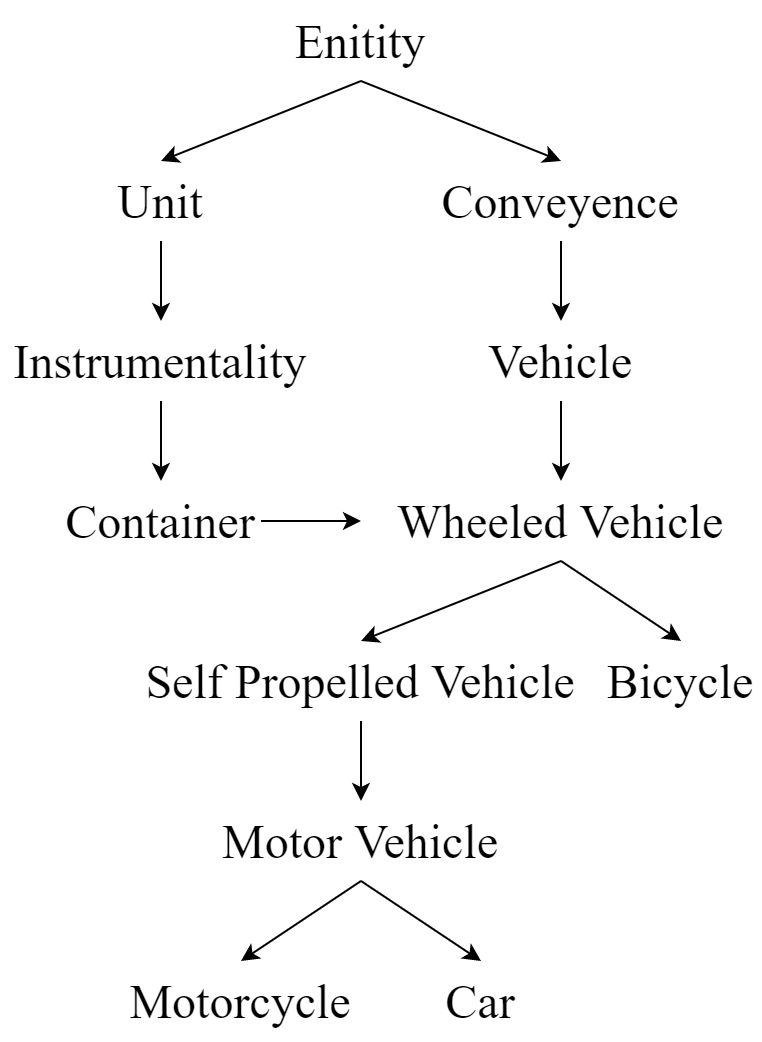
\includegraphics[width=250px]{WordNet.png}
  \caption[Hierarchical Structure of WordNet]{Figure shows the hierarchical structure from WordNet.}
  \label{fig:wordnet}
\end{figure}

% 同義詞詞林由 Mei \emph{et al}. 完成,收錄了五萬三千多個詞。因年代久遠,許多用詞與現在已經差異很大,後來由 HIT 修編為同義詞詞林擴增版,擴增為七萬多個詞,並放在由 HIT 所建立的 Language Technology Platform Cloud 上供大家下載與研究。
\paragraph{}
Tongyici Cilin (or Chinese Synonym Forest, 同義詞詞林) written by Mei \emph{et al}. \cite{mei1983hit} in 1983, which has collected over 53k words. Nowadays, some words have become less used, and many modern words appear. Therefore, the Harbin Institute of Technology Information Retrieval Lab (HIT IR Lab)\footnote{http://ir.hit.edu.cn/} extended Tongyici Cilin to collected over 70k words and removed both the old words and the uncommon words. The Extended Tongyici Cilin is provided on the Language Technology Platform Cloud\footnote{https://www.ltp-cloud.com/} build by HIT for people to download and research.

\paragraph{}
The original Tongyici Cilin provides three levels of encoding to represent the synset. Level 1 using an upper letter, level 2 using a lower letter, and a two-digit number for level 3. There are additional level 4 and level 5 in Extended Tongyici Cilin to represent the finer granularity of the synsets as shown in Table \ref{table:tc_encoding}. An upper letter for level 4, and a two-digit number for level 5. The rank of the level is higher, the granularity is finer.

\paragraph{}
Figure \ref{fig:tc_sample} shows the examples of Tongyici Cilin. The level 1 encoding ``B'' is entity category, so the encoding of list begins with ``B'' is a list of entity words, like \texttt{Bf02A02=} and \texttt{Bg01A08@}. The level 1 encoding ``C'' is location category, so the encoding begins with ``C'' is a list of location words, like \texttt{Cb06E09@}.

\paragraph{}
The level 2 encoding ``Bf'' represents that the list of words is related to ``rain''. The level 3 encoding ``Bf02'' represents that the list of words is related to ``wind''. We can see that the encoding level is more similar, the group of the words is closer.

\paragraph{}
There is a category symbol follow by each encoding. ``='' represents that the words are synonyms. ``\#'' means that the words in the group are related. ``@'' indicates that the list only contains one word.

\begin{figure}[H]
  \centering
  \caption{Examples of Extended Tongyici Cilin}
  \begin{minipage}{\linewidth}
    \centering
    \setlength{\extrarowheight}{-3pt}
    \begin{tabular}{ll}
    Encoding & Words \\ \hline
    \texttt{Bf02A02=} & 大風\ 疾風\ 狂風\ 暴風\ 扶風 \\
    \texttt{Bf02A03=} & 颶風\ 颱風\ 強風\ 飈\ 強颱風 \\
    \texttt{Bf02B02=} & 雲氣\ 靄 \\
    \texttt{Bf04B02\#} & 朝霞\ 晚霞\ 煙霞 \\
    \texttt{Bg01A08@} & 溫水 \\
    \texttt{Cb06E09@} & 民間 \\
    \end{tabular}
    \label{fig:tc_sample}
  \end{minipage}
\end{figure}

\begin{table}[H]
  \centering
  \setlength{\extrarowheight}{-3pt}
  \begin{tabular}{|l|C{1.1cm}|C{1.1cm}|C{1.1cm}|C{1.1cm}|C{1.1cm}|C{1.1cm}|C{1.1cm}|C{1.1cm}|}
  \hline
  Digits & 1 & 2 & 3 & 4 & 5 & 6 & 7 & 8 \\ \hline
  Example & D & a & 1 & 5 & B & 0 & 2 & =\#@ \\ \hline
  Level & Lv1 & Lv2 & \multicolumn{2}{c|}{Lv3} & Lv4 & \multicolumn{2}{c|}{Lv5} &  \\ \hline
  \end{tabular}
  \caption{Extended Tongyici Cilin encoding table.}
  \label{table:tc_encoding}
\end{table}

\paragraph{}
We use the WUP similarity \cite{wu-palmer-1994-verb} in WordNet to construct semantic features. The WUP similarity of synset is defined as Eq(\ref{eq:wup_synset}). $s_1$ and $s_2$ means the synset of a word. $lcs$ means the least common subsumer of the $s_1$ and $s_2$. $depth$ is the length of the synset to the root.

\begin{equation} \label{eq:wup_synset}
  wup_{synset}(s_1,s_2)=\frac{2\times depth(lcs)}{depth(s_1)+depth(s_2)}
\end{equation}

\paragraph{}
Since each word may have more than one synset, we defined the WUP similarity of word in Eq(\ref{eq:wup_word}). We calculate all the WUP similarities between all the synsets of the word $w_1$ and the word $w_2$. The maximum will be the word WUP similarity of $w_1$ and $w_2$.

\begin{equation} \label{eq:wup_word}
  wup_{word}(w_1,w_2)=\max\limits_{\substack{s_1\in synsets(w_1) \\ s_2\in synsets(w_2)}} wup_{synset}(s_1,s_2)
\end{equation}

\paragraph{}
We utilize NLTK (Natural Language Toolkit) \cite{nltk} to calculate the WUP similarity.

\paragraph{}
We use the Tongyici Cilin to build the lv5 similarity calculation system. The lv5 similarity of synset defined as Eq(\ref{eq:lv5_synset}). Given a synset $s_1$ and a synset $s_2$, we use $level$ to calculate the common level of $s_1$ and $s_2$, and then divide by five.

\begin{equation} \label{eq:lv5_synset}
  lv5_{synset}(s_1, s_2)=level(s_1,s_2)/5
\end{equation}

\paragraph{}
Since each word may linked by more than one synset in Tongyici Cilin, we defined the word-level lv5 similarity in Eq(\ref{eq:lv5_word}).

\begin{equation} \label{eq:lv5_word}
  lv5_{word}(w_1,w_2)=\max\limits_{\substack{s_1\in synsets(w_1) \\ s_2\in synsets(w_2)}} lv5_{synset}(s_1,s_2)
\end{equation}

\paragraph{}
% 因為中文的部份缺少完善的 WordNet 資源,而英文的部份則是缺少同義詞詞林的資源,所以這部份會透過 Cosine Similarity 來取代。
We lack a proper WordNet resource in Chinese due to the existing Chinese WordNet is outmoded, it is unable to calculate the WUP similarity in Chinese since it will encounter too many missing words. And there is no similar resources of Tongyici Cilin in English, it is unable to calculate the lv5 similarity in English. They will be replaced with the cosine similarity. Given the word vectors $A$ and $B$, the cosine similarity is defined as Eq(\ref{eq:cos_sim}).

\begin{equation} \label{eq:cos_sim}
  sim_{cos}(A, B)=\frac{A\cdot B}{||A||\ ||B||}=\frac{\sum\limits^{n}_{i=1}A_iB_i}{\sqrt{\sum\limits^{n}_{i=1}A^2_i}\sqrt{\sum\limits^{n}_{i=1}B^2_i}}
\end{equation}

\paragraph{}
The average of the WUP similarity is defined in Eq(\ref{eq:average_wup}). The average of the lv5 similarity is defined in Eq(\ref{eq:average_lv5}). The cosine similarity is defined in Eq(\ref{eq:average_cos_sim}). $t_1$ and $t_2$ is the words of the premise and the hypothesis respectively. We sum the maximum and then divide by the total number of the words of $t_1$.

\begin{equation} \label{eq:average_wup}
  avg_{wup}(t_1,t_2)=\frac{1}{|t_1|}\sum\limits_{w_1\in t_1}\max\limits_{w_2\in t_2}wup_{word}(w_1, w_2)
\end{equation}

\begin{equation} \label{eq:average_lv5}
  avg_{lv5}(t_1,t_2)=\frac{1}{|t_1|}\sum\limits_{w_1\in t_1}\max\limits_{w_2\in t_2}lv5_{word}(w_1, w_2)
\end{equation}

\begin{equation} \label{eq:average_cos_sim}
  avg_{cos}(t_1,t_2)=\frac{1}{|t_1|}\sum\limits_{W_1\in t_1}\max\limits_{W_2\in t_2}sim_{cos}(W_1, W_2)
\end{equation}

\paragraph{}
Note that no matter in any type of similarity, we only consider the content words of the sentences.

\paragraph{}
The semantic features in English are listed as follows:

\begin{enumerate}
  \item[17.] average cosine similarity $(t_1)$
  \item[18.] average cosine similarity $(t_2)$
  \item[19.] average WUP similarity $(t_1)$
  \item[20.] average WUP similarity $(t_2)$
\end{enumerate}

\paragraph{}
The semantic features in Chinese are listed as follows:

\begin{enumerate}
  \item[17.] average cosine similarity $(t_1)$
  \item[18.] average cosine similarity $(t_2)$
  \item[19.] average lv5 similarity $(t_1)$
  \item[20.] average lv5 similarity $(t_2)$
\end{enumerate}

\subsubsection{Sentence Embedding}
\paragraph{}
% 因為句對間的蘊含關係有時並不需要用到整句話的資訊,只需要部份資訊,因此 Sentence Embedding 這種呈現 sentence features 的方法就是個不錯的選擇。Sentence Embedding 是由 Word Embedding 的向量計算而來,而關於 Word Embedding 的詳細敘述,請參考 Word Embedding 章節。在本論文中,我們選擇使用單純的總和平均做為計算 Sentence Embedding 的方法。
Another straightforward method to convert one sentence into one vector is to find the arithmetic mean of the embedding vectors of all the words in the sentence. The detailed discussion of word embedding is given in the Sec. \ref{section:word_embedding}.

\paragraph{}
After calculating sentence embedding vectors of the premise and the hypothesis in a pair from the RTE dataset, the real input to the neural network is the concatenation of these two embedding vectors.

\subsection{Word-based Sequence Input} \label{section:word_embedding}
\paragraph{}
The second kind of approaches to represent a sentence is to generate a sequence of word representations. For neural networks, a word is often represented as an embedding vector. The sequence of word embedding vectors can be the input of RNN or BERT.

\subsubsection{Raw Text Input}
\paragraph{}
% 在自然語言領域裡使用深度學習時,經常使用將每個字詞表達成一組向量的方法,將這組詞向量根據句子做排列而得到的詞向量序列做為神經網路的輸入層特徵。而在 RTE 任務裡,我們將 Premise 和 Hypothesis 串接起來,並在中間加入一個特殊 Token <SEP> 做為區隔。用來表達詞向量的方法有很多種,我們將在接下來的章節介紹這些語言模型。
When using deep learning in the field of natural language process, it is common to represent each word as a vector and combined it as a sequence of word vectors according to the order of the sentence, this word-based sequence will be the input features of the neural network. In the recognizing textual entailment task, we concatenated the sequence of word vectors of the premise and the hypothesis, a special token ``\texttt{[SEP]}'' will be put in the middle as the separator. There are many methods to represent the word embedding, we will introduce them in the following sections.

\subsubsubsection{Self-Trained Word Embedding}
\paragraph{}
% 與 Pre-trained Word Embedding 不同,Self-trained Embedding 通常做為神經網路的其中一個 Layer,並透過神經網路的梯度傳導機制不斷調整每個字詞的向量,根據任務的方向去學習適當的權重。Pre-trained Word Embedding 通常只會適合 Pretraining 時所使用的文本領域,若是 Pretraining 時的文本領域不夠廣泛或過於特殊,可能會對實驗效能有不好的影響。但因為 Self-trained Word Embedding 可以根據任務文本去進行彈性調整,所以在特定領域可能會有更好的表現,但也有可能因為資料數量不足的關係而使效能有所限制。
Different from the pre-trained word embedding, self-trained embedding usually use as a layer of a neural network and adjust each word vector through the backpropagation mechanism of the neural network. To the pre-trained word embedding, the suitable task is limited by the pre-training corpus. If the pre-training corpus is not common enough, it might have a bad influence on the experiments. The self-trained word embedding can do flexible adjustment according to the domain of the task text, therefore the performance may be better in a certain domain, but also may be limited by the data size of the training dataset.

\subsubsubsection{fastText}
\paragraph{}
fastText \cite{bojanowski2016enriching} is a library for efficient text classification and representation learning created by Facebook's AI Research (FAIR) lab. This library allows us to create word embedding with unsupervised learning algorithms, like skip-gram and continuous bag-of-word (CBOW). With this library, we train a word representation from Traditional Chinese Wikipedia, both in the version of skip-gram and CBOW. The dimension of the word embedding is 250.

\subsubsubsection{Google NNLM}
\paragraph{}
Google NNLM is provided by TensorFlow Hub\footnote{https://www.tensorflow.org/hub} which has many different language models that already be trained by a large corpus. We use the Chinese version of NNLM that trained on Simplified Chinese Google News 100B corpus and publish by Google\footnote{https://tfhub.dev/google/tf2-preview/nnlm-zh-dim128/1}. In order to fit the Traditional Chinese dataset, we convert the dictionary of the Google NNLM from Simplified Chinese into Traditional Chinese.
% BERT Language Model

\subsubsection{Similarity-based Word Sequence} \label{section:csa}
% 指的是 CSA 但要講得比現在版本更清楚、要想像
\paragraph{}
We propose a new approach called similarity-based word sequence (SWS hereafter). This approach creates a new sequence of words (SWS) from two sentences according to the word alignment based on semantic similarity. The leading part of SWS contains semantically similar (aligned) words. The trailing part of SWS contains un-aligned (semantically dissimilar) words. The embedding vector of a word in SWS is the subtraction of the embedding vectors of the aligned words.

\paragraph{}
We expect SWS can be useful in RTE task. For a bidirectional entailment pair, most of the words can be aligned to their corresponding similar word, and the subtraction of their embedding vectors will be close to zero vector. For a forward entailment pair, the trailing part of SWS contains certain amount of un-aligned content words, therefore the entailment is one-directional. For an independent pair, both the premise and the hypothesis have content words that cannot be aligned.

\paragraph{}
If a contradiction pair is related to antonyms, at least one pair of un-aligned words are antonyms, and their vector subtraction can be identified by the neural network. If a contradiction pair is related to negations, one of the un-aligned words will be the negation word, and it may be recognized by the neural network.

\paragraph{}
Details and examples are given as follows. Figure \ref{fig:sws_b} shows an alignment result of a bidirectional entailment sentence pair, most of the words are aligned. Figure \ref{fig:sws_f} shows an alignment result of a forward entailment sentence pair, most of the words in the hypothesis are aligned, but some content words of the premise are not aligned. Figure \ref{fig:sws_i} shows an alignment result of an independence sentence pair, most of the words are un-aligned.

% B
% 有時候 生產商 會 在 鉛筆 的 一 端 裝上 橡皮擦
% 有時候 鉛筆 的 一 端 會 被 生產商 裝上 橡皮擦
\hspace*{-1.5in}
\begin{figure}[H]
  \centering
  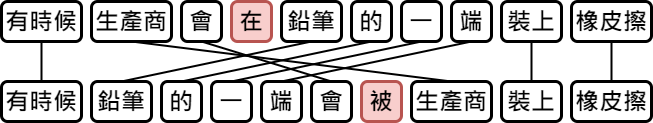
\includegraphics[scale=0.6]{SWS.B.png}
  \caption[SWS Bidirectional Entailment Example]{SWS bidirectional entailment example.}
  \label{fig:sws_b}
\end{figure}

% F
% 約瑟夫·傅立葉 是 十九世紀 法國 數學家 、 物理學家
% 約瑟夫·傅立葉 是 物理學家
\hspace*{-1.5in}
\begin{figure}[H]
  \centering
  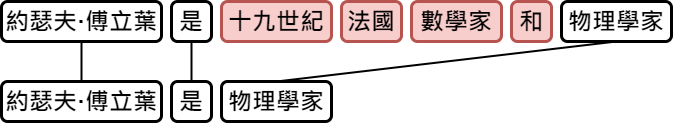
\includegraphics[scale=0.6]{SWS.F.png}
  \caption[SWS Forward Entailment Example]{SWS forward entailment example.}
  \label{fig:sws_f}
\end{figure}

% I
% 鉛筆 的 原型 可以 追溯 至 古羅馬 時代
% 羅馬人 發明 鉛筆
\hspace*{-1.5in}
\begin{figure}[H]
  \centering
  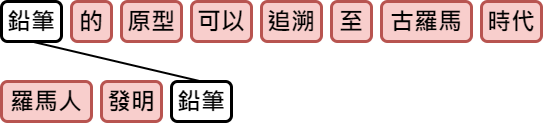
\includegraphics[scale=0.6]{SWS.I.png}
  \caption[SWS Independence Example]{SWS independence example.}
  \label{fig:sws_i}
\end{figure}

\paragraph{}
Figure \ref{fig:sws_c_antonym} shows an alignment result of a contradiction sentence pair related to antonym. Un-aligned words are antonyms. Figure \ref{fig:sws_c_neg} shows an alignment result of a contradiction sentence pair related to negation, the negation word is un-aligned.

% C Antonym
% 東協 自由 貿易 區 於 1992年 提出
% 東協 自由 貿易 區 於 1992年 撤銷
\hspace*{-1.5in}
\begin{figure}[H]
  \centering
  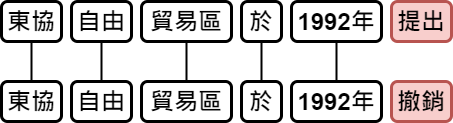
\includegraphics[scale=0.6]{SWS.C.Antonym}
  \caption[SWS Antonym Contradiction Example]{SWS antonym contradiction example.}
  \label{fig:sws_c_antonym}
\end{figure}

% C Negation
% 喬治·盧卡斯 最 著名 的 作品 是 《 星際 大戰 》 和 《 法櫃 奇兵 》 系列
% 喬治·盧卡斯 最 著名 的 作品 不 是 《 星際 大戰 》 和 《 法櫃 奇兵 》 系列
\begin{figure}[H]
  \centering
  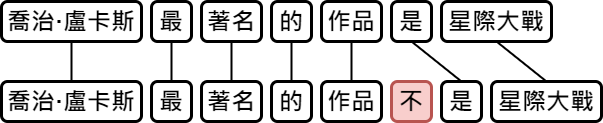
\includegraphics[scale=0.6]{SWS.C.Negation.png}
  \caption[SWS Negation Contradiction Example]{SWS negation contradiction example.}
  \label{fig:sws_c_neg}
\end{figure}

% o align the words by calculating the cosine similarity between the premise and the hypothesis. We will have a argument ``similarity threshold'' to define if the two words will be aligned. We will decide the similarity threshold in the experiment of the threshold argument tuning.

\paragraph{}
We align the words based on the cosine similarity. We have a argument ``similarity threshold'' to control whether the words will be aligned. Figure \ref{fig:sim_threshold} shows an example that two different words are aligned since their cosine similarity is higher than the threshold. This threshold will be decide by the experiment of the argument tuning.

\hspace*{-1.5in}
\begin{figure}[H]
  \centering
  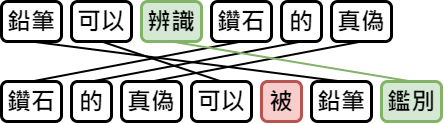
\includegraphics[scale=0.6]{Threshold.png}
  \caption[SWS Alignment Result with Threshold]{Alignment result of similarity-based word sequence.}
  \label{fig:sim_threshold}
\end{figure}

% 首先先計算兩句話的每個詞之間的 Cosine Similarity 建立一個 Similarity Table,然後從表中挑出相似數值最高的兩個詞,將 premise 的詞放入 list1 並將 hypothesis 的詞放入 list2,然後將這兩個詞從表中刪去,再繼續往下挑相似數值最高的兩個詞,直到該相似數值小於 Similarity Threshold 為止。接下來把 premise 剩下的詞一個一個放入 list1,每放一個詞到 list1 裡面,就在 list2 裡面放一個零,hypothesis 剩下的詞也是一樣的操作。最後將 list2 的值減去 list1 獲得最後的 CSA Features。
% To calculate the similarity-based word sequence, we will first calculate the cosine similarity of each word of two sentences to build a similarity table. Then picked up the word pair with the highest value of similarity, and put the word vector of the word from the premise sentence into $list_1$ and put the one from the hypothesis sentence into $list_2$. Then remove the two words from the similarity table. Repeat this step until the highest value of the similarity is lower than the similarity threshold. Next, we put the word vectors of the left words of the premise sentence into $list_1$ one by one. Every time we put a word vector into $list_1$, put a zero vector into $list_2$, and do the same operation to the left words of the hypothesis sentence. Therefore the two lists will remain the same size. After all, we use $list_2$ to minus $list_1$ to obtain the final ``SWS Features''.

% \begin{figure}[H]
%   \centering
%   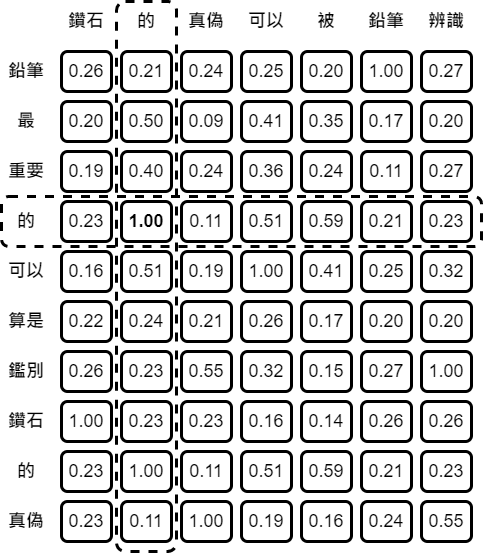
\includegraphics[width=250px]{WAG.png}
%   % 此圖顯示兩句話裡每個字之間的 Cosine Similarity,每個字將會根據這個 Cosine Similarity Table 進行 Alignment
%   \caption[Cosine Similarity Table]{Cosine similarity table.}
%   \label{fig:csa}
% \end{figure}

% \begin{figure}[H]
%   \centering
%   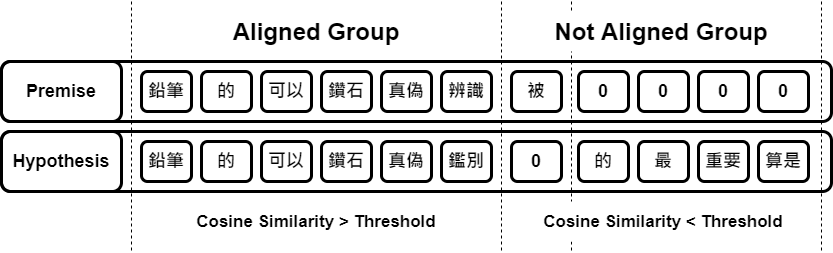
\includegraphics[width=\textwidth]{Groups.png}
%   % 此圖顯示兩句話裡每個字之間的 Cosine Similarity,每個字將會根據這個 Cosine Similarity Table 進行 Alignment
%   \caption[Alignment Result of Similarity-based Word Sequence]{Alignment result of similarity-based word sequence.}
%   \label{fig:wag_groups}
% \end{figure}

\section{Transfer Learning and Data Expansion} \label{section:pseudo}

\paragraph{}
Many researches of deep learning in recent years mentioned that the scale of training data size has a huge impact on the performance of the system. RTE datasets are often constructed in a large scale. As we can see, the number of pairs in MNLI is 433k and the number of pairs in CNLI is 100k.

\paragraph{}
However, the number of pairs in the RITE2 training set is only 1,321 and it is only 581 in the RITE-VAL training set. The amount of the training data is extremely insufficient for deep learning. Therefore, we adopt two approaches, transfer learning and data expansion, to conquer the problem of data insufficiency.

\subsection{Transfer Learning Using Other NLI Datasets} \label{section:add_other_nli}

\paragraph{}
The transfer learning technique uses a larger training set constructed either for another domain, under a different definition of task, or in another language to pre-train a classifier, and then use the training set of the main task to fine-tune the classifier.

\paragraph{}
We use several available RTE datasets to build classifiers for RITE tasks by transfer learning, including MNLI, CNLI, and OCNLI. We also try to merge two datasets to become a larger training set.

\paragraph{}
But these datasets were constructed in different languages. MNLI is in English, and both CNLI and OCNLI are in Chinese. Since CNLI and OCNLI are in the same language with RITE, the monolingual language models can be used for pre-training, such as our pre-trained Chinese word embedding model or BERT.

\paragraph{}
To use training sets written in different languages, we need to choose a multilingual language model. Fortunately, BERT also provide a multilingual version. We can use the multilingual BERT to train a model by MNLI, a dataset in English, and then fine-tune the model with a RITE training set written in Chinese.

\paragraph{}
We follow two approaches to further expand the training sets. The first is to merge MNLI and CNLI to become a larger dataset (named as MixNLI hereafter). The second approach is two-step pre-training. We first pre-train the model with MNLI, and then pre-train the model with CNLI. These pre-trained models are further fine-tuned by the RITE training sets.

% We can use different languages of datasets at the same time through the technique of cross-lingual transfer learning. We have two approaches to reach the purpose. The first is to mix MNLI and CNLI to become a new dataset, we called this dataset MixNLI. The second is two-steps pre-training. We first pre-train the model with MNLI, then second pre-train the model with CNLI.

\paragraph{}
Labels (entailment classes) defined in MNLI or CNLI datasets are different from the ones defined in RITE. MNLI and CNLI are ECN tasks, which means that the labels are ``entailment'', ``contradiction'', and ``neutral''. However, RITE tasks are BFCI tasks, which means that the labels are ``bidirectional entailment'', ``forward entailment'', ``contradiction'', and ``independence''. We need to find a method to convert ECN labels into BFCI labels.

\paragraph{}
Comparing the two label sets, ``contradiction'' is the same in both sets, and ``neutral'' can be map into ``independence'' directly. In order to decide whether an ``entailment'' pair is ``bidirectional entailment'' or ``forward entailment'', we try to build a good ECN classifier for each NLI dataset to automatically decide the entailment relations of the NLI pairs in the reverse direction.

\paragraph{}
Given an ``entailment'' pair, the two sentences in the pair are exchanged, i.e. the premise becomes the hypothesis and the hypothesis becomes the premise. We then use the ECN classifier to decide its label. If it is ``entailment'', it means that the entailment is in both direction, thus the final label is ``bidirectional entailment''. On the other hand, if the label of the reversed pair is ``neutral'', it means that the entailment only in one direction, thus the final label is ``forward entailment''. In rare cases, the reversed pair is mis-classified into ``contradiction''. We ignore such result and assign the label of the pair as ``forward entailment''.

\subsection{Reversed Labeling}
\label{sec:revlabel}
\paragraph{}
To expand the RITE datasets, we utilize the additional information of reversed labels of the RITE-VAL dataset. When the premise and the hypothesis exchanged, the entailment relation will changed. The reversed labels means the entailment relation of the reversed sentence pairs.

\paragraph{}
We add the reversed pairs into RITE-VAL, and called this dataset as RITE-Extended. The data size of RITE-Extended is 1,103. We also mix it with RITE2 to become a new training data. We called this dataset RITE-Extended-v2. The total size of RITE-Extended-v2 is 2,292.

\subsection{Generation-based Data Expansion}
% 我們嘗試使用大量的虛擬資料來改進模型的效能,虛擬資料的產生方式則有規則式改寫與 GPT-2 模型生成兩種。這兩種方法會對四個標籤都產生等量的資料,並根據 MNLI 的資料量,各產生 400k 組句對。在接下來的章節會介紹產生虛擬資料的細節。
\label{section:pseudo_dataset}
\paragraph{}
We attempt to automatically create large-scale pseudo datasets to improve the performance of textual entailment recognition. We propose two approaches to generate the pseudo data, including rule-based rewriting and GPT-2 generation. Both methods will generate equal amount of data for four labels. To be comparable with the MNLI dataset, the set of pairs in each label will be expanded to 400k.

\subsubsection{Rule-Based RTE Pair Generation}
% \subsubsection{CIRB}
% CIRB, Synonym Dictionary, Antonym Dictionary, Negation Words
% 首先我們先介紹產生虛擬訓練資料會需要用到的資源。因為產生虛擬資料的方法基本上是透過改寫句子得來的,而改寫規則未必能夠適用於任何句子上,因此我們需要有足夠大量的文章才能確保生成的句子數量是充足的。CIRB (Chinese Information Retrieval Benchmark) 是一份來自 NTCIR 2 資訊檢索子任務的測試集,蒐集了 1998 年到 2005 年間五家線上新聞媒體的新聞文章資料,總共 280 萬篇文章,每篇文章的長度平均為 560 個字,包含的領域廣泛分佈於政治、財經、體育、娛樂、科技、國際等。且 RITE 資料集本身也有一些句子是來自於新聞文章,所以我們認為 CIRB 是一個相當合適的資料集。
\label{para:cirb}
\paragraph{}
We design several rewriting rules to generate RTE pairs, including synonym/antonym substitution and negation insertion. Long sentences can be further divided to create new sentences. These methods are explained as follows.

\subsubsubsection*{Synonym/Antonym substitution}
\paragraph{}
Given a sentence in Chinese natural language, we randomly pick a word in the sentence which have synonyms or antonyms in the dictionary, and replace the word with one of its synonyms or antonyms randomly.

\paragraph{}
Assume that a word $w$ in a sentence $S$ is substituted and the sentence $S$ becomes $S'$, if the word $w$ is substituted with its synonym, $S$ and $S'$ still have the same meaning, thus $(S,S')$ is a ``bidirectional entailment'' pair. On the other hand, if the word $w$ is substituted with its antonym, $S$ and $S'$ will have antonymous meanings, thus $(S,S')$ is a ``contradiction'' pair.

\paragraph{}
We use the synonym dictionary and the antonym dictionary to generate the pseudo training data. The synonym dictionary can be built by using the Tongyici Cilin base on the well-organized synonym encoding. And the Academia Sinica Bilingual Ontological WordNet (Sinica BOW) \cite{huang2004sinica} can be used to build the antonym dictionary.

\paragraph{}
Sinica BOW is a thesauri that integrates the English WordNet 1.6 and the Chinese WordNet. Figure \ref{fig:bow} shows the example data of Sinica BOW. We can see that the record of the Sinica BOW is built based on the synset offset of WordNet. We can easily build the Chinese antonym dictionary by the antonym information in WordNet with these mapping records from Sinica BOW.

\begin{figure}
  \centering
  \caption{The example of the Academia Sinica Bilingual Ontological WordNet.}
  \begin{minipage}{\linewidth}
    \begin{lstlisting}[language=XML]
    <Record Count="171509">
      <EnglishLemma>deep</EnglishLemma>
      <POS>Adverb</POS>
      <WordNetSynsetOffset Version="1.6">00300307</WordNetSynsetOffset>
      <EnglishFrequancyRank>#通用詞彙#</EnglishFrequancyRank>
      <ChineseTransList>
        <ChineseTrans>
          <ChineseLemma>#深入地#</ChineseLemma>
        </ChineseTrans>
      </ChineseTransList>
    </Record>
    <Record Count="171510">
      <EnglishLemma>deep</EnglishLemma>
      <POS>Adjective</POS>
      <WordNetSynsetOffset Version="1.6">00654761</WordNetSynsetOffset>
      <EnglishFrequancyRank>#通用詞彙#</EnglishFrequancyRank>
      <ChineseTransList>
        <ChineseTrans>
          <ChineseLemma>#深的#</ChineseLemma>
        </ChineseTrans>
      </ChineseTransList>
    </Record>
    \end{lstlisting}
  \end{minipage}
  \label{fig:bow}
\end{figure}

\subsubsubsection*{Negation Insertion}
\paragraph{}
Given a sentence with no negation words, we try to find the best position to insert a negation word according to a part-of-speech trigram probabilistic model. The list of negation words comes from
Tongyici Cilin.

\paragraph{}
To apply this rule, we have to prepare a negation-related part-of-speech trigram probabilistic model. First, we collect sentences with negation words in a large corpus. Second, these sentences are POS-tagged by CKIP tagger \footnote{https://github.com/ckiplab/ckiptagger}\cite{Li_Fu_Ma_2020} and all words except negation words are replaced with their POS. Trigrams where the second word is a negation word are extracted for further calculation. Note that the marks of sentence boundaries are added at the beginning and in the end of sentences before trigram extraction.

% negation-context frequency
\paragraph{}
Bigrams consisting of the first and the third POS in these negation-centered trigrams are extracted and counted. We define the frequency of such a bigram as its \textbf{\emph{negation-context frequency}}. Given a POS-tagged sentence, an occurrence of a POS bigram with a high negation-context frequency indicates that it is likely to appear a negation word in the middle of the bigram. We simply choose the POS bigram with a highest negation-context frequency and insert a negation word in the middle. The sentences before and after the negation insertion form a new ``contradiction'' pair.

\paragraph{}
The choice of the inserted negation word is random but according to the ratio of the occurrence of negation words. For a POS bigram, we collect the negation-centered trigrams which generate this POS bigram, and count the frequency of each negation word appearing in the center. The probability of a negation word to be inserted is proportional to its frequency in these trigrams.

% ('Na', 'Nb'): '否': 90, '非': 10
% ('Na', 'Nc'): '否': 10, '非': 990

\subsubsubsection*{Sentence Splitting}
\paragraph{}
We use a straightforward method to create ``forward entailment'' pairs. That is, we choose sentences containing one or more commas and divide it into several sub-sentences according to the commas. The original sentence and any one of its sub-sentences can produce a ``forward entailment'' pair.

\paragraph{}
This method can be also applied to the new pairs generated by the previous two rules. Given a rule-generated pair $(t_1,t_2)$, $t_1$ can be paired with any sub-sentence of $t_2$ to become a new RTE pair. If the sub-sentence contains a synonym, the label of the new pair is ``forward entailment''. If the sub-sentence contains an antonym, the label of the new pair is ``contradiction''. If the sub-sentence contains a newly inserted negation word, the label of the new pair is ``contradiction''. Otherwise, the label of the new pair is ``forward entailment''.

\subsubsubsection*{Random Selection}
\paragraph{}
Finally, we randomly choose two sentences from the large corpus to produce a new RTE pair and assign its label as ``independence''. Table \ref{example:sim_nli_rule_based} shows the examples of sentence pair generated by rule-based generation.

\paragraph{}
\paragraph{}
Obviously, we need a large corpus to pick sentences for RTE pair generation and to measure the negation-context frequencies. We merge all the CIRB corpora to become a large corpus for this purpose.

% \paragraph{}
% First, we introduce the resources used in the generation of pseudo training data. Most of the generated data come from the modification of sentences and the rewriting rules may not be applied to any sentences, so we need to ensure the number of the articles is enough to generate sufficient sentences.

\paragraph{}
The CIRB (Chinese Information Retrieval Benchmark) \cite{chen2001cirb} dataset is a test collection of the Chinese information retrieval tasks of NTCIR 2 which collected the news articles released from the websites of Chinatimes\footnote{https://www.chinatimes.com/}, Chinatimes Commercial\footnote{https://ctee.com.tw/}, Chinatimes Express, Central Daily News, and China Daily News during 1998 to 2005.

\paragraph{}
There are in total 2.8 million articles with an average length of 560 characters. The domains covered are widely distributed in politics, finance, sports, entertainment, technology, and international. Besides, the part of sentences in the RITE dataset also comes from the news article. We believe that the CIRB collection is a suitable corpus for our purpose.

\begin{table}[H]
  \centering
  \setlength{\extrarowheight}{-3pt}
  \begin{tabular}{|l|l|c|}
    \hline
    \multicolumn{1}{|c|}{Method} & \multicolumn{1}{c|}{Sentence Pair} & Label \\ \hline
    \multirow{2}{*}{Synonym} & 失控所致或營造而成,差異極大 & \multirow{2}{*}{B} \\ \cline{2-2}
    & 失控所致或營造而成,反差極大 &  \\ \hline
    \multirow{2}{*}{Synonym \& Split (1)} & 失控所致或營造而成,差異極大 & \multirow{2}{*}{F} \\ \cline{2-2}
    & 失控所致或營造而成 &  \\ \hline
    \multirow{2}{*}{Synonym \& Split (2)} & 失控所致或營造而成,差異極大 & \multirow{2}{*}{F} \\ \cline{2-2}
    & 反差極大 &  \\ \hline
    \multirow{2}{*}{Antonym} & 即日起上市,可預約宅配 & \multirow{2}{*}{C} \\ \cline{2-2}
    & 即日起上市,不許預約宅配 &  \\ \hline
    \multirow{2}{*}{Antonym \& Split (1)} & 即日起上市,可預約宅配 & \multirow{2}{*}{F} \\ \cline{2-2}
    & 即日起上市 &  \\ \hline
    \multirow{2}{*}{Antonym \& Split (2)} & 即日起上市,可預約宅配 & \multirow{2}{*}{C} \\ \cline{2-2}
    & 不許預約宅配 &  \\ \hline
    \multirow{2}{*}{Negation} & 相較之下,台灣藝術家以公共藝術文化輸出的案例卻未聽聞 & \multirow{2}{*}{C} \\ \cline{2-2}
    & 相較之下,台灣藝術家以非公共藝術文化輸出的案例卻未聽聞 &  \\ \hline
    \multirow{2}{*}{Negation \& Split} & 相較之下,台灣藝術家以公共藝術文化輸出的案例卻未聽聞 & \multirow{2}{*}{C} \\ \cline{2-2}
    & 台灣藝術家以非公共藝術文化輸出的案例卻未聽聞 &  \\ \hline
    \multirow{2}{*}{Independence} & 也許真的自古英雄多寂寞,女人也不例外 & \multirow{2}{*}{I} \\ \cline{2-2}
    & 這個週期「魔咒」,誰也掙脫不了 &  \\ \hline
  \end{tabular}
  \caption{Example of sentence pair generated by rule-based methods.}
  \label{example:sim_nli_rule_based}
\end{table}

\subsubsection{GPT-2 Generation}
% GPT-2 \cite 是由 OpenAI 所開發的一個自然語言產生模型,在機器翻譯、問答、總結和文本產生都有相當出色的表現。而透過 GPT-2 模型產生虛擬資料的這個實驗,我們參考了 _ 論文中的做法,從 Corpus 中隨機挑選句子,並將非內容詞去除,只留下內容詞做為「head seed」,然後將完整的句子拼接在 head seed 後面,目的是訓練 GPT-2 模型在餵入這些內容詞後,可以產生完整的句子。在適當的訓練下,對 GPT-2 模型餵入相同的內容詞做為 head seed 可以產生不同但相似的句子。
\paragraph{}
GPT-2 \cite{radford2019language} is a natural language generation model created by OpenAI. It has an excellent performance in machine translation, question answering, summarization, and text generation. The GPT-2 generation method of the simulation dataset is based on Hegde \emph{et al}. \cite{hegde2020unsupervised}.

\paragraph{}
We randomly picked sentences from the corpus and removed the non-content word, only remain the content words as the seeds of GPT-2. Then we concatenated the original sentence after the seeds. We use special tokens \texttt{[CLS]} and \texttt{[SEP]} to surround the seed. Therefore, the model can distinguish the boundary of the seeds and the sentence.

\paragraph{}
Our purpose is to train the GPT-2 model that can generate a complete sentence including the words of the seeds. With proper training, the GPT-2 model can generate different but similar sentences from the same seeds.

% 我們保留訓練資料中的原句做為 Premise,並使用相同的 head seed 產生一個句子做為 Hypothesis ,這樣獲得的句對可以標記為 B。接下來,我們透過更換 head seed 的內容詞來產生其他不同標記的句對。從 head seed 中隨機挑選兩個詞並互換位置,這樣產生的句對為 B。將 head seed 中的部份內容詞去除,這樣產生的句對為 F。從 head seed 中隨機挑選一個內容詞變成反義詞,這樣產生的句對為 C。隨機插入一個否定詞在 head seed 裡面,產生出來的句對為 C。只保留一個 head seed 的內容詞,並隨機放入其他內容詞,產生出來的句對為 I。
\paragraph{}
We keep the original sentence of the training example as the premise sentence and use the same seeds from the training example to generate a new sentence as the hypothesis sentence. These sentence pairs will be labeled as ``bidirectional''.

\paragraph{}
Next, we generate sentences for different labels by changing the word of seeds. We randomly pick one word and replace it with synonym. The generated sentence pairs will be labeled as ``bidirectional''. We randomly pick two words of seeds and exchanged their position. The generated sentence pairs will be labeled as ``bidirectional''.

\paragraph{}
We randomly remove one to three words of seeds, the generated sentence pairs will be labeled as ``forward entailment''. We randomly pick one content word and replace it with an antonym, the generated sentence pairs will be labeled as ``contradiction''.

\paragraph{}
We randomly insert a negation word in seeds, the generated sentence pairs will be labeled as ``contradiction''. At last, only remain one content word of seeds and put three to ten random words within, the generated sentence pairs will be labeled as ``independence''. Table \ref{example:GPT-2_pseudo} shows the examples of the GPT-2 pseudo sentences.

\begin{table}[H]
  \centering
  \setlength{\extrarowheight}{-3pt}
  \begin{tabular}{|l|l|l|c|}
  \hline
  \multicolumn{1}{|c|}{Method} & \multicolumn{1}{c|}{Seed} & \multicolumn{1}{c|}{Generated Sentence} & Label \\ \hline
  Original & {[}CLS{]} 無 理性 能力 {[}SEP{]} & 以致無理性思考的能力。 & - \\ \hline
  Same & {[}CLS{]} 無 理性 能力 {[}SEP{]} & 是極端無理性的能力。 & B \\ \hline
  Exchange & {[}CLS{]} 理性 無 能力 {[}SEP{]} & 只有理性和無能力。 & B \\ \hline
  Synonym & {[}CLS{]} 非 理性 能力 {[}SEP{]} & 也是非理性能力的一種。 & B \\ \hline
  Remove & {[}CLS{]} 無 能力 {[}SEP{]} & 還是無能力了! & F \\ \hline
  Antonym & {[}CLS{]} 所有 理性 無資格 {[}SEP{]} & 或是所有理性的人都無資格。 & C \\ \hline
  Negation & {[}CLS{]} 非 理性 無 能力 {[}SEP{]} & 一般是非理性、無能力 & C \\ \hline
  Random & {[}CLS{]} 出發 能力 表達 清楚 {[}SEP{]} & 出發雖有能力,但卻表達不清楚。 & I \\ \hline
  \end{tabular}
  \caption{Example of sentence generated by GPT-2.}
  \label{example:GPT-2_pseudo}
\end{table}

% 我們使用 CIRB 做為 Corpus,並根據四個標籤平均生成資料集,每個標籤下的每一種方法也同樣生成平均數量的資料。規則式與 GPT-2 根據 MNLI 的資料集規模,各自生成四十萬組句對,總共生成八十萬組句對。
\paragraph{}
We generate the dataset equally according to the four labels, each generation method also generates an equal number of data under each label. Both rule-based and GPT-2 generate 400k sentence pairs respectively. Both scale of the training set is similar to MNLI, result in an 800k sentence pairs pseudo training dataset. Table \ref{table:pseudo_training_data_dist} shows the distribution of the pseudo training dataset.

\begin{table}[H]
  \centering
  \setlength{\extrarowheight}{-3pt}
  \begin{tabular}{|l|l|c|r|c|}
  \hline
  \multicolumn{1}{|c|}{System} & \multicolumn{1}{c|}{Method} & Label & \multicolumn{1}{c|}{Number} & Total \\ \hline
  \multirow{10}{*}{Rule-Based} & Synonym & B & 100k & \multirow{10}{*}{400k} \\ \cline{2-4}
   & Antonym & C & 25k &  \\ \cline{2-4}
   & Negation Word & C & 25k &  \\ \cline{2-4}
   & Antonym and Split (1) & C & 25k &  \\ \cline{2-4}
   & Negation Word and Split (1) & C & 25k &  \\ \cline{2-4}
   & Synonym and Split & F & 33k &  \\ \cline{2-4}
   & Antonym and Split (2) & F & 33k &  \\ \cline{2-4}
   & Negation Word and Split (2) & F & 33k &  \\ \cline{2-4}
   & Radom Pick & I & 50k &  \\ \cline{2-4}
   & Random Split & I & 50k &  \\ \hline
  \multirow{7}{*}{GPT-2} & Same Seed & B & 33k & \multirow{7}{*}{400k} \\ \cline{2-4}
   & Synonym & B & 33k &  \\ \cline{2-4}
   & Exchange Position & B & 33k &  \\ \cline{2-4}
   & Random Remove & F & 100k &  \\ \cline{2-4}
   & Antonym & C & 50k &  \\ \cline{2-4}
   & Negation Word & C & 50k &  \\ \cline{2-4}
   & Remain One & I & 100k &  \\ \hline
  \end{tabular}
  \caption{The pseudo training data distribution.}
  \label{table:pseudo_training_data_dist}
\end{table}

\section{Experiments} \label{section:experiments}
\subsection{Datasets and Evaluation Metrics}
\paragraph{}
% ?? 解釋使用 F1 的原因 (Unbalanced Label)
% 根據 NTCIR 主辦單位提供的正式評估公式來計算 macroF1
According to the formal evaluation formula provided by NTCIR:

\begin{equation}
  macroF1=\frac{1}{|C|}\sum_{c\in C}F1_c
\end{equation}

\paragraph{}
$C$ is all categories, and $c$ is one of the categories. Because $macroF1$ is the average of F1-Score to each category, it would not be affected by a category that has a large number. The experiments of the BFCI task will use this evaluation formula.

\paragraph{}
F-measure also called F1-score, is a measure that is calculated from precision and recall. It is usually used in the information retrieval field to compare the different systems. F1-score, precision, and recall are defined as follows.

\begin{equation}
  F1=\frac{2\times Precision\times Recall}{Precision+Recall}
\end{equation}

\begin{equation}
  Precision=\frac{N_{correct}}{N_{predicted}}
\end{equation}

\begin{equation}
  Recall=\frac{N_{correct}}{N_{target}}
\end{equation}

\paragraph{}
% 在 RITE 的實驗中,我們對 Training Set 進行 10-Fold Cross-validation,並計算這十個 Fold 的 Micro F1-Score 做為評估結果之一。而測試集的部份則以 10-Fold 產生出來的 10 個權重各評估一次並取平均做為 Test F1-Score。
In the experiments of RITE, we do the 10-fold cross-validation to the training set and calculate the micro F1-score as one of the evaluation results. We evaluate the test set by each model weight of the ten folds, then take the average as test F1-score.

\paragraph{}
To compare the experiments of the ECN tasks with the other systems, we use accuracy as the evaluation formula of the ECN tasks.

\paragraph{}
To understand the impact of the characters of the Traditional and the Simplified, we use OpenCC\footnote{https://github.com/BYVoid/OpenCC} which available as a python package to convert CNLI and OCNLI into CNLI-TW and OCNLI-TW. The original CNLI and OCNLI in Simplified Chinese will be called CNLI-CN and OCNLI-CN.

\subsection{Machine Learning Feature Experiments}
% 首先我們重製了 Liu 等人的 SVM 實驗,並與 MLP 做比較。在 Scikit-Learn 套件中提供了四個 Kernel: RBF, Linear, Sigmoid, and Poly,所以我們先比較了不同的 SVM Kernel。
% 在 Liu 等人的實驗中,分別將 Lexical (lex), Syntactic (syn), Word Similarity (wn), 與 Synonym Forest (cl) 各自去除,來測試哪個特徵對實驗結果的影響較大。而在 MLP 的實驗中,我們也做了相同的步驟。
% 接下來,我們嘗試用基本的 RNN Model 來進行實驗。RNN 的部份測試了 LSTM 與 GRU 以及各自加上 Attention 的效果,在 Word Embedding 的部份則測試了 Self-trained, fastText CBOW, fastText Skip-gram, 與 GoogleNNLM。其結果如表:(待補)
% (st/ftCBOW/ftSG/g x LSTM/GRU x with/without Attention)
% 在這個實驗的基礎上,我們將 ML Features 結合到 RNN Model 裡面。我們將 RNN Encoder 的 Output 與 ML Features 做 Concatenate 後再進行分類,其結果如表(待補)
% 而在本論文中,我們提出了 CSA 方法,並將 CSA 特徵放入 RNN Model,也分別測試了與 ML Features 或 Word Embedding 做結合的實驗,其結果如表:(待補)
% \paragraph{}
% To cross-compare the performance of datasets, we first extended the RITE-VAL with reversed labels to generate RITE-VAL-REV and mixed RITE2 with RITE-VAL-REV to generate RITE-VAL-REV-2. So we have RITE2, RITE-VAL, RITE-VAL-REV, and RITE-VAL-REV-2 to be used as the training sets. The test sets of RITE2 and RITE-VAL will be called as RITE2-TEST and RITE-VAL-TEST.

\paragraph{}
% SVM 的實驗結果:Kernel Comparison
We use SVM provide by the Scikit-Learn package. Since the Scikit-Learn package provides four types of kernels of SVM: RBF, Linear, Sigmoid, and Poly, we must decide the most suitable kernel for our experiment of SVM. Therefore, we use the machine learning features mentioned in Sec. \ref{section:ml_features} to compare the performance of the different kernels of SVM. In this experiment, we used RITE-Extended-v2 that mentioned in Sec. \ref{sec:revlabel} as the training set. The results are shown in Table \ref{svm_kernel}. We can see that the performance of kernel RBF is outperformed all the other kernels except the RITE2 test set. Therefore, the RBF kernel will be chosen as the main kernel in the following experiments.

\begin{table}[H]
  \centering
  \setlength{\extrarowheight}{-3pt}
  \caption{Results of the SVM kernels comparison.}
  \label{svm_kernel}
  \begin{tabular}{|l|r|r|r|r|}
  \hline
  \multicolumn{1}{|c|}{\multirow{2}{*}{Kernel}} & \multicolumn{2}{c|}{RITE-VAL} & \multicolumn{2}{c|}{RITE2} \\ \cline{2-5}
  \multicolumn{1}{|c|}{} & \multicolumn{1}{c|}{Dev} & \multicolumn{1}{c|}{Test} & \multicolumn{1}{c|}{Dev} & \multicolumn{1}{c|}{Test} \\ \hline
  RBF & \textbf{0.4011} & \textbf{0.3674} & \textbf{0.5177} & 0.4099 \\ \hline
  Linear & 0.3538 & 0.3017 & 0.4872 & \textbf{0.4474} \\ \hline
  Sigmoid & 0.2696 & 0.2386 & 0.3126 & 0.2550 \\ \hline
  Poly & 0.3495 & 0.3363 & 0.4949 & 0.4386 \\ \hline
  \end{tabular}
\end{table}

\paragraph{}
We are interested in different feature combination of the machine learning features. We use feature selection by manual removing the certain features in the machine learning features to observe the changes of performance. The feature selection is given as follows.

\begin{table}[H]
  \centering
  \setlength{\extrarowheight}{-3pt}
  \begin{tabular}{ll}
    $all$ & all of the features will be used. \\
    $all-f_{lex}$ & the n-gram features will be removed. \\
    $all-f_{syn}$ & the syntactic features will be removed. \\
    $all-f_{cos}$ & the cosine similarity features of semantic features will be removed. \\
    $all-f_{sim}$ & the lv5 similarity and WUP similarity of semantic features will be removed. \\
  \end{tabular}
\end{table}

\paragraph{}
Table \ref{result:ft_select} shows the results. We can see that $all-f_{cos}$ have better performance on RITE-VAL. Though it is not the best in RITE2, but it is not too bad. Therefore, we choose $all-f_{cos}$ as the main machine learning features combination for SVM.

\begin{table}[H]
  \centering
  \setlength{\extrarowheight}{-3pt}
  \caption{Comparison of the feature selection using SVM.}
  \label{result:ft_select}
  \begin{tabular}{|l|l|l|l|l|}
  \hline
  \multicolumn{1}{|c|}{\multirow{2}{*}{Feature}} & \multicolumn{2}{c|}{RITE-VAL} & \multicolumn{2}{c|}{RITE2} \\ \cline{2-5}
  \multicolumn{1}{|c|}{} & \multicolumn{1}{c|}{Dev} & \multicolumn{1}{c|}{Test} & \multicolumn{1}{c|}{Dev} & \multicolumn{1}{c|}{Test} \\ \hline
  all & \textbf{0.3840} & \textbf{0.3522} & 0.5220 & 0.4527 \\ \hline
  all-lex & 0.3701 & 0.3428 & 0.4913 & 0.4119 \\ \hline
  all-syn & 0.3673 & 0.2839 & \textbf{0.5572} & 0.4386 \\ \hline
  all-cos & 0.3829 & 0.3500 & 0.4965 & 0.4566 \\ \hline
  all-sim & 0.3746 & 0.3294 & 0.5450 & \textbf{0.4616} \\ \hline
  \end{tabular}
\end{table}

\paragraph{}
We also do the feature selection on MLP. Table \ref{result:ft_select_mlp} shows the results. We can see that $all$ have a better performance overall. Therefore, $all$ is chosen to be the main machine learning features for MLP.

\begin{table}[H]
  \centering
  \setlength{\extrarowheight}{-3pt}
  \caption{Comparison of the feature selection using MLP.}
  \label{result:ft_select_mlp}
  \begin{tabular}{|l|l|l|l|l|}
  \hline
  \multicolumn{1}{|c|}{\multirow{2}{*}{Feature}} & \multicolumn{2}{c|}{RITE-VAL} & \multicolumn{2}{c|}{RITE2} \\ \cline{2-5}
  \multicolumn{1}{|c|}{} & \multicolumn{1}{c|}{Dev} & \multicolumn{1}{c|}{Test} & \multicolumn{1}{c|}{Dev} & \multicolumn{1}{c|}{Test} \\ \hline
  all & 0.4107 & 0.3506 & \textbf{0.4665} & \textbf{0.4625} \\ \hline
  all-lex & \textbf{0.4146} & 0.3504 & 0.4479 & 0.4321 \\ \hline
  all-syn & 0.3726 & 0.2822 & 0.4355 & 0.4478 \\ \hline
  all-cos & 0.4134 & \textbf{0.3523} & 0.4641 & 0.4488 \\ \hline
  all-sim & 0.4098 & 0.3516 & 0.4653 & 0.4512 \\ \hline
  \end{tabular}
\end{table}

\paragraph{}
% 當 Training Source 是 RITE-VAL 的時候,MLP 的效能可能不見得是最好的,我們認為這可能是因為 RITE-VAL 的資料規模相對較小,在資料規模不大的情況下 SVM 可以取得較好的效果。
We compare the performance of SVM and MLP. We use the original dataset as the training data. Note the SVN using the features $all-cos$ and MLP using the features $all$. The results are shown in Table \ref{result:ml_original}. We can see that SVM have better performance in test set, while MLP have better performance in development set. We think this is caused by the overfitting of MLP since the size of the training sets is not enough.

\paragraph{}
Through Table \ref{result:ml_original}, we can also observe that when using the RITE2 training data, the performance always gets better. Since the original data size of RITE2 is double than the data size of RITE-VAL, we think the size of data may be a critical role.

\begin{table}[H]
  \centering
  \setlength{\extrarowheight}{-3pt}
  \caption{Comparing of SVM and MLP including inter-dataset validation.}
  \label{result:ml_original}
  \begin{tabular}{|c|l|r|r|r|r|}
  \hline
  \multirow{2}{*}{System} & \multicolumn{1}{c|}{\multirow{2}{*}{Training}} & \multicolumn{2}{c|}{RITE-VAL} & \multicolumn{2}{c|}{RITE2} \\ \cline{3-6}
   & \multicolumn{1}{c|}{} & \multicolumn{1}{c|}{Dev} & \multicolumn{1}{c|}{Test} & \multicolumn{1}{c|}{Dev} & \multicolumn{1}{c|}{Test} \\ \hline
  \multirow{2}{*}{SVM} & RITE-VAL & 0.3829 & 0.3500 & 0.3441 & 0.3273 \\ \cline{2-6}
   & RITE2 & 0.4290 & \textbf{0.4965} & 0.3435 & \textbf{0.4566} \\ \hline
  \multirow{2}{*}{MLP} & RITE-VAL & 0.4107 & 0.3506 & 0.3655 & 0.3261 \\ \cline{2-6}
   & RITE2 & \textbf{0.4665} & 0.3715 & \textbf{0.5936} & 0.4512 \\ \hline
  \end{tabular}
\end{table}

% \begin{table}[H]
%   \centering
%   \setlength{\extrarowheight}{-3pt}
%   \begin{tabular}{|l|R{2.5cm}|R{2.5cm}|R{2.5cm}|R{2.5cm}|}
%   \hline
%   Training Source & \multicolumn{2}{c|}{RITE-VAL} & \multicolumn{2}{c|}{RITE2} \\ \hline
%   Classifier & \multicolumn{1}{c|}{SVM} & \multicolumn{1}{c|}{MLP} & \multicolumn{1}{c|}{SVM} & \multicolumn{1}{c|}{MLP} \\ \hline
%   Validation Target & \multicolumn{4}{c|}{RITE-VAL Dev} \\ \hline
%   $all$ & \textbf{0.3840} & 0.4107 & 0.4203 & \textbf{0.4665} \\ \hline
%   $all - lex$ & 0.3701 & \textbf{0.4146} & 0.3864 & 0.4479 \\ \hline
%   $all - syn$ & 0.3673 & 0.3726 & 0.4100 & 0.4355 \\ \hline
%   $all - cos$ & 0.3829 & 0.4134 & \textbf{0.4290} & 0.4641 \\ \hline
%   $all - sim$ & 0.3746 & 0.4098 & 0.4211 & 0.4653 \\ \hline
%   Validation Target & \multicolumn{4}{c|}{RITE2 Dev} \\ \hline
%   $all$ & 0.3639 & 0.3655 & 0.5220 & 0.5936 \\ \hline
%   $all - lex$ & 0.3733 & 0.3590 & 0.4913 & 0.5654 \\ \hline
%   $all - syn$ & 0.3289 & 0.3457 & \textbf{0.5572} & 0.5516 \\ \hline
%   $all - cos$ & 0.3441 & 0.3598 & 0.4965 & 0.5820 \\ \hline
%   $all - sim$ & \textbf{0.3864} & \textbf{0.3752} & 0.5450 & \textbf{0.5954} \\ \hline
%   Validation Target & \multicolumn{4}{c|}{RITE-VAL Test} \\ \hline
%   $all$ & \textbf{0.3522} & 0.3506 & 0.3427 & \textbf{0.3715} \\ \hline
%   $all - lex$ & 0.3428 & 0.3504 & 0.3537 & 0.3584 \\ \hline
%   $all - syn$ & 0.2839 & 0.2822 & 0.3375 & 0.3016 \\ \hline
%   $all - cos$ & 0.3500 & \textbf{0.3523} & 0.3435 & 0.3709 \\ \hline
%   $all - sim$ & 0.3294 & 0.3516 & \textbf{0.3598} & 0.3702 \\ \hline
%   Validation Target & \multicolumn{4}{c|}{RITE2 Test} \\ \hline
%   $all$ & 0.3413 & \textbf{0.3261} & 0.4527 & 0.4512 \\ \hline
%   $all - lex$ & 0.3319 & 0.3130 & 0.4119 & 0.4321 \\ \hline
%   $all - syn$ & 0.3455 & 0.3033 & 0.4386 & 0.4478 \\ \hline
%   $all - cos$ & 0.3273 & 0.3197 & 0.4566 & 0.4488 \\ \hline
%   $all - sim$ & \textbf{0.3559} & 0.3196 & \textbf{0.4616} & \textbf{0.4625} \\ \hline
%   \end{tabular}
%   \caption{Results of SVM and MLP comparison using original training data.}
%   \label{result:ml_original}
% \end{table}

\subsection{Sentence-Based Embedding Experiments}
% 在 Sentence-based embedding 的實驗中,我們將 Self-Trained Word Embedding, fastText CBOW, fastText Skip-gram 與 Google NNLM 等四種 NNLM 分別進行測試,sentence embedding 的算法為 word embedding 的平均,其結果如表。可見 fastText CBOW 的效果較好,我們認為這是 CBOW 的特性使得這個 NNLM 相當適合進行 Sentence Embedding 的實驗。
In the experiments of sentence-based embedding, we test the four types of word embeddings mentioned in Sec. \ref{section:word_embedding}. The calculation of sentence embedding is the average of the word embedding of the sentence. We used MLP to test the performance. The results are shown in Table \ref{result:sent_emb_nnlm}. We can see that the performance of fastText CBOW is the best. It might because of the mechanism of the CBOW calculation to make this word embedding suitable with the experiments of sentence embedding.

\begin{table}[H]
  \centering
  \setlength{\extrarowheight}{-3pt}
  \caption{Results of the different word embedding in the experiment of sentence embedding.}
  \label{result:sent_emb_nnlm}
  \begin{tabular}{|l|l|l|l|l|}
  \hline
  \multicolumn{1}{|c|}{\multirow{2}{*}{Word   Embedding}} & \multicolumn{2}{c|}{RITE-VAL} & \multicolumn{2}{c|}{RITE2} \\ \cline{2-5}
  \multicolumn{1}{|c|}{} & \multicolumn{1}{c|}{Dev} & \multicolumn{1}{c|}{Test} & \multicolumn{1}{c|}{Dev} & \multicolumn{1}{c|}{Test} \\ \hline
  Self-trained & 0.1382 & 0.1000 & 0.2711 & 0.1445 \\ \hline
  fastText CBOW & \textbf{0.3335} & \textbf{0.2551} & \textbf{0.3818} & 0.2755 \\ \hline
  fastText Skip-gram & 0.2631 & 0.1550 & 0.3623 & \textbf{0.2762} \\ \hline
  Google NNLM & 0.2363 & 0.1874 & 0.1851 & 0.2019 \\ \hline
  \end{tabular}
\end{table}

\subsection{Word-Based Embedding Experiments}
\subsubsection{Raw Text Input Experiments}
\paragraph{}
In the raw text input experiments, we first use the RAD model to test each type of word embeddings. The results are shown in Table \ref{result:nnlm_comparison}. The self-trained word embedding seems to have good performance in the development set, but not the performance in the test set. The word embeddings that come from fastText are performed well in both the development set and test set, and the fastText skip-gram is better than the fastText CBOW. Therefore, the fastText skip-gram will be chosen as our main word embedding in the following experiments.

\begin{table}[H]
  \centering
  \setlength{\extrarowheight}{-3pt}
  \begin{tabular}{|l|l|l|l|l|}
  \hline
  \multicolumn{1}{|c|}{\multirow{2}{*}{Word   Embedding}} & \multicolumn{2}{c|}{RITE-VAL} & \multicolumn{2}{c|}{RITE2} \\ \cline{2-5}
  \multicolumn{1}{|c|}{} & \multicolumn{1}{c|}{Dev} & \multicolumn{1}{c|}{Test} & \multicolumn{1}{c|}{Dev} & \multicolumn{1}{c|}{Test} \\ \hline
  Self-trained & \textbf{0.4334} & 0.3611 & 0.2203 & 0.2495 \\ \hline
  fastText CBOW & 0.3982 & 0.3662 & 0.2106 & 0.2343 \\ \hline
  fastText Skip-gram & 0.3882 & \textbf{0.3801} & \textbf{0.2445} & \textbf{0.2715} \\ \hline
  Google NNLM & 0.2788 & 0.2922 & 0.1961 & 0.2549 \\ \hline
  \end{tabular}
  \caption{Comparison of different word embeddings.}
  \label{result:nnlm_comparison}
\end{table}

\paragraph{}
We want to determine which layer arrangement of the recurrent neural network is better. We tried the different combinations of the neural network composed of the layers above. We use ``R'' for short of ``Recurrent Neural Network'', ``A'' for short of ``Attention Layer'', ``D'' means ``Fully-connected Dense Layer'', also known as output layer. The results are shown in Table \ref{result:nn_types_comparison}. The RAD model has the best performance in the test set, and there is only a small gap of performance in the development set with other model types. This result shows that a recurrent neural network layer followed by an attention layer is a better combination of layer arrangement of the model. Therefore, we will use the RAD model as our main model type of recurrent neural network.

\begin{table}[H]
  \centering
  \setlength{\extrarowheight}{-3pt}
  \begin{tabular}{|l|l|l|l|l|}
  \hline
  \multicolumn{1}{|c|}{\multirow{2}{*}{Model}} & \multicolumn{2}{c|}{RITE-VAL} & \multicolumn{2}{c|}{RITE2} \\ \cline{2-5}
  \multicolumn{1}{|c|}{} & \multicolumn{1}{c|}{Dev} & \multicolumn{1}{c|}{Test} & \multicolumn{1}{c|}{Dev} & \multicolumn{1}{c|}{Test} \\ \hline
  RAD & 0.3882 & \textbf{0.2445} & 0.3801 & \textbf{0.2715} \\ \hline
  ARD & \textbf{0.3933} & 0.2098 & 0.3631 & 0.2292 \\ \hline
  RD & 0.3928 & 0.2148 & \textbf{0.3837} & 0.2580 \\ \hline
  AD & 0.3307 & 0.1895 & 0.3333 & 0.2133 \\ \hline
  \end{tabular}
  \caption{Comparison of different layer arrangements of recurrent neural networks.}
  \label{result:nn_types_comparison}
\end{table}

% 比較 RNN Types
\paragraph{}
% RNN 有多種變形,藉由 Tensorflow API 我們可以使用三種基本的 RNN 形式:Vanilla RNN, LSTM, 與 GRU,我們將這三種 RNN 做比較,得到表的結果。可見 GRU 與 LSTM 的效果差距很小,因為 GRU 所需消耗的訓練資源比較低,所以我們選擇 GRU 做為主要的 RNN Layer。
We compare three variants of the recurrent neural network. We build these basic types of recurrent neural networks through Tensorflow API. We also compare the BERT model with these three types of RNN layers and acquired the results of Table \ref{result:rnn_types}. We can see that BERT outperforms all the other models. The differences between LSTM and GRU are slight. Due to the advantage of the lower resource cost of GRU, we choose GRU as the main RNN layer.

\begin{table}[H]
  \centering
  \setlength{\extrarowheight}{-3pt}
  \begin{tabular}{|l|l|l|l|l|}
  \hline
  \multirow{2}{*}{Neural Network} & \multicolumn{2}{c|}{RITE-VAL} & \multicolumn{2}{c|}{RITE2} \\ \cline{2-5}
   & \multicolumn{1}{c|}{Dev} & \multicolumn{1}{c|}{Test} & \multicolumn{1}{c|}{Dev} & \multicolumn{1}{c|}{Test} \\ \hline
  Vanilla RNN & 0.3716 & 0.2196 & 0.3337 & 0.2399 \\ \hline
  LSTM & \textbf{0.4408} & \textbf{0.2276} & 0.3816 & 0.2494 \\ \hline
  GRU & 0.4316 & 0.2197 & \textbf{0.3828} & \textbf{0.2578} \\ \hline
  BERT & \textbf{0.4907} & \textbf{0.3767} & \textbf{0.5582} & \textbf{0.4403} \\ \hline
  \end{tabular}
  \caption{Results of the different neural networks.}
  \label{result:rnn_types}
\end{table}

\subsubsection{Word-Alignment Experiments}
\paragraph{}
We introduce the ``Similarity-based Word Sequence'' in the Sec. \ref{section:csa}. We need to decide the argument ``Cosine Similarity Threshold'' first. We tune the argument from 0.1 to 1.0 with step 0.1. We use the RAD model in this experiment. The results are shown in Table \ref{result:threshold_comparison} and the trend plotted in Figure \ref{fig:threshold}. This figure shows the trend of the performance with different cosine similarity thresholds in each dataset. We can see the performance gets better with the cosine similarity to get increased. The performances between 0.8 to 1.0 are much better than the other intervals, and 0.8 seems the common higher point overall. Therefore, we decide to choose 0.8 as the cosine similarity threshold.

\begin{figure}[H]
  \centering
  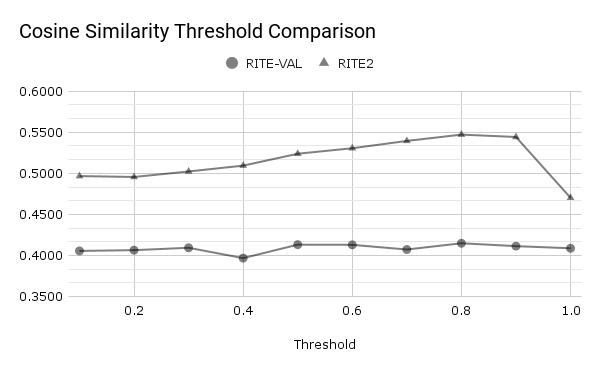
\includegraphics[width=15cm]{SimThresholdComp.png}
  \caption[Cosine Similarity Threshold Comparison]{The comparison of the cosine similarity threshold of the similarity-based word sequence.}
  \label{fig:threshold}
\end{figure}

\begin{table}[H]
  \centering
  \setlength{\extrarowheight}{-3pt}
  \caption{The detailed performance of the comparison of the cosine similarity threshold.}
  \label{result:threshold_comparison}
  \begin{tabular}{|c|r|r|r|r|}
  \hline
  \multirow{2}{*}{Threshold} & \multicolumn{2}{c|}{RITE-VAL} & \multicolumn{2}{c|}{RITE2} \\ \cline{2-5}
   & \multicolumn{1}{c|}{Dev} & \multicolumn{1}{c|}{Test} & \multicolumn{1}{c|}{Dev} & \multicolumn{1}{c|}{Test} \\ \hline
  0.1 & 0.4188 & 0.3455 & 0.4894 & 0.3440 \\ \hline
  0.2 & 0.4032 & 0.3314 & 0.4992 & 0.3564 \\ \hline
  0.3 & 0.4144 & 0.3223 & 0.5023 & 0.3523 \\ \hline
  0.4 & 0.3967 & 0.3210 & 0.5094 & 0.4058 \\ \hline
  0.5 & 0.4161 & 0.3041 & 0.5239 & 0.4030 \\ \hline
  0.6 & 0.4134 & 0.3137 & 0.5306 & 0.3837 \\ \hline
  0.7 & 0.4116 & 0.3109 & 0.5352 & 0.3795 \\ \hline
  0.8 & 0.4223 & 0.3419 & 0.5413 & 0.3720 \\ \hline
  0.9 & 0.4062 & 0.3137 & 0.5415 & 0.4015 \\ \hline
  1.0 & 0.4010 & 0.3510 & 0.5442 & 0.3853 \\ \hline
  \end{tabular}
\end{table}

\paragraph{}
We want to know the performance of the similarity-based word sequence combines with machine learning features. We use an augmented RAD model to concatenate the machine learning features with the hidden states of similarity-based word sequence. The results are shown in Table \ref{result:csa_nn}. Most of the performances are better than the neural network input by similarity-based word sequence only. This result proves that the machine learning features are beneficial to the systems.

\begin{table}[H]
  \centering
  \setlength{\extrarowheight}{-3pt}
  \caption{Comparison of the features in the neural network.}
  \label{result:csa_nn}
  \begin{tabular}{|l|l|l|l|l|}
  \hline
  \multicolumn{1}{|c|}{\multirow{2}{*}{Feature}} & \multicolumn{2}{c|}{RITE-VAL} & \multicolumn{2}{c|}{RITE2} \\ \cline{2-5}
  \multicolumn{1}{|c|}{} & \multicolumn{1}{c|}{Dev} & \multicolumn{1}{c|}{Test} & \multicolumn{1}{c|}{Dev} & \multicolumn{1}{c|}{Test} \\ \hline
  SWS Only & 0.4062 & 0.3137 & \textbf{0.5415} & 0.4015 \\ \hline
  SWS   + ML Features & \textbf{0.4283} & \textbf{0.3364} & 0.5407 & \textbf{0.4069} \\ \hline
  \end{tabular}
\end{table}

\subsection{Experiments with Transfer Learning}
\paragraph{}
In this experiment, we first reproduce the performance of BERT on the MNLI dataset. We use \texttt{bert-base-uncased} model. The learning rate is 3e-5. After two epochs of training, the accuracy of the development set is 0.8346, which is close to the original paper (0.846). Then we reproduce the same experiment of the BERT model on the OCNLI dataset. We used the \texttt{bert-base-chinese} model since it is a Chinese dataset. The accuracy of the development set is 0.7447, which is also close to the original paper (0.745). After reproducing these two experiments successfully, we applied the same experiment on the CNLI dataset. The accuracy of the development set of CNLI is 0.7830, and the accuracy of the test set is 0.7832. Though the performance is not better than the best system in CCL 2018 (0.8238), the performance is better than the second-best system (0.7828).

\paragraph{}
% 首先我們以 CNLI 做為 pre-training data 並以 RITE 進行 fine-tune。
We use the CNLI dataset as the training data first, then test on RITE2 and RITE-VAL directly. The BERT model we fine-tuned is \texttt{bert-base-chinese}. The results are shown in Table \ref{result:bert_compare} as the baseline system \#1. We can see that the performance of this baseline system is much better than the best system in either Liu \emph{et al}. or the NTCIR conference.

\begin{table}[H]
  \centering
  \setlength{\extrarowheight}{-3pt}
  \begin{tabular}{|c|l|r|r|r|r|}
  \hline
  \multirow{2}{*}{\#} & \multicolumn{1}{c|}{\multirow{2}{*}{System}} & \multicolumn{2}{c|}{RITE-VAL} & \multicolumn{2}{c|}{RITE2} \\ \cline{3-6}
   & \multicolumn{1}{c|}{} & \multicolumn{1}{c|}{Dev} & \multicolumn{1}{c|}{Test} & \multicolumn{1}{c|}{Dev} & \multicolumn{1}{c|}{Test} \\ \hline
  1 & CNLI-TW-Only & 0.4766 & 0.4993 & 0.5377 & 0.5950 \\ \hline
  2 & CNLI-TW & 0.5915 & 0.5146 & 0.6848 & 0.6426 \\ \hline
  3 & CNLI-CN & 0.5609 & 0.4977 & 0.6724 & 0.6293 \\ \hline
  4 & MNLI & 0.5713 & \textbf{0.5561} & 0.6919 & \textbf{0.7107} \\ \hline
  5 & OCNLI-TW & 0.5316 & 0.5092 & 0.6710 & 0.5884 \\ \hline
  6 & MNLI \& CNLI & 0.5811 & \textbf{0.5650} & 0.6952 & 0.6955 \\ \hline
  7 & MixNLI & 0.5895 & \textbf{0.5592} & 0.6880 & \textbf{0.7036} \\ \hline
  8 & MNLI + ML Features & 0.5216 & 0.5301 & 0.6697 & \textbf{0.7032} \\ \hline
  \end{tabular}
  \caption{Results of the BERT that train with the different datasets.}
  \label{result:bert_compare}
\end{table}

\paragraph{}
% 藉由上個實驗的成功,我們進一步的將 RITE 切成 10-fold 並納入 fine-tune 的環節,我們將 CNLI 訓練出來的模型透過每個 fold 的 training set 再進行一次訓練,並測試該 fold 的 test set,最後將每個 fold 的測試集結果合併在一起進算 micro f1。得到的結果如表 x,其效能有大幅度的提昇。
We introduce transfer learning by pretraining the BERT model with the additional datasets and fine-tuning it with the RITE datasets. We split the RITE dataset into fixed 10-folds. The label conversion of ECN to BFCI is described in Sec. \ref{section:add_other_nli}. We use the CNLI-TW dataset to pre-trained the BERT model. Then we use the training set of the remaining folds to fine-tune and test by the test set of the target fold. Then we merge the results of all folds and calculated the micro f1-score. The results are shown in Table \ref{result:bert_compare} as the system \#2. We can see that the performance has a huge improvement through this training technique.

\paragraph{}
We also compare the performance between CNLI-CN and CNLI-TW. The system \#3 in Table \ref{result:bert_compare} is the results of CNLI-CN. We can see that the performance of CNLI-TW is better than CNLI-CN. We think the dataset composed of Traditional Chinese characters is more suitable for RITE. This result proves that the conversion from Simplified Chinese to Traditional Chinese is helpful to the system.

\paragraph{}
Next, we use the cross-lingual transfer learning to train the \texttt{bert-multilingual-cased} model. Since this model is the multilingual version of the BERT model, we can directly fine-tune with the different languages of the datasets. In this experiment, we used the MNLI dataset to pre-train the model and then fine-tune it with the RITE datasets. Since the scale of the MNLI dataset is four times larger than the CNLI, we excepted the performance will be better. The results are shown in Table \ref{result:bert_compare} as the system \#4. We can see that the performance has a huge improvement. The test F1-score of RITE-VAL became over 55\%, and the test F1-score of RITE2 even breakthrough 70\%.

\paragraph{}
% 我們同樣進行了以 OCNLI 為訓練資料的實驗,OCNLI 的句子品質相較於 CNLI 而言較高一點,但其資料規模並不如 CNLI。以同樣的方法進行實驗之後,其實驗結果如表。結果顯示,以 OCNLI 為訓練集的實驗,無論在 RITE2 或 RITE-VAL 的實驗上,效能皆不如以 CNLI 作為訓練集的實驗。
The OCNLI dataset claimed that their sentences have better quality, but the amount of data is only half of the CNLI dataset. We are also curious about the performance of this dataset, which has higher sentence quality with lower data size. We use the Traditional Chinese version of OCNLI (OCNLI-TW). The results are shown in Table \ref{result:bert_compare} as the system \#5. We can see that the performance is not much better than the system \#2 or the system \#3.

\paragraph{}
% 我們試著將 CSA 與 ML Features 這兩種方法與 BERT 模型做結合。與 CSA 結合的部份,我們先透過一層 RNN 進行 Encoding 然後與 BERT Hidden State 拼接在一起進行輸出,而 ML Features 的部份則是直接拼接並進行輸出,最後還有將三者做結合的實驗,並以 CNLI 做為 benchmark。其實驗結果如表,從 RITE-VAL 的角度來看,加入 CSA 與 ML Features 的做法並沒有帶來正面的提昇,而從 RITE2 的角度而言,效能的提昇也是相當微幅。可見 BERT 所能學習到的特徵表示是相當深入的。
We try to combine the BERT model with the similarity-based word sequence and the machine learning features to see how these features will impact the performance. We use the CNLI-TW dataset as the benchmark. In the combination of similarity-based word sequence, we first encode the similarity-based word sequence features with a recurrent neural network layer and concatenate them with BERT hidden states to output. In the machine learning features, we concatenate the features with BERT hidden states directly. Finally, we concatenate three of them for comparison. The results are shown in Table \ref{result:bert_csa_mlft_comparison}. No matter the similarity-based word sequence, machine learning features, or both of them have no significant improvement to the RITE-VAL. Only have a little improvement to the RITE2. We can see that the feature representation that the BERT model can learn is quite in-depth.

\begin{table}[H]
  \centering
  \setlength{\extrarowheight}{-3pt}
  \caption{Results of the BERT using machine learning features and similarity-based word sequence.}
  \label{result:bert_csa_mlft_comparison}
  \begin{tabular}{|l|l|l|l|l|}
  \hline
  \multicolumn{1}{|c|}{\multirow{2}{*}{System}} & \multicolumn{2}{c|}{RITE-VAL} & \multicolumn{2}{c|}{RITE2} \\ \cline{2-5}
  \multicolumn{1}{|c|}{} & \multicolumn{1}{c|}{Dev} & \multicolumn{1}{c|}{Test} & \multicolumn{1}{c|}{Dev} & \multicolumn{1}{c|}{Test} \\ \hline
  Original & 0.4766 & 0.4993 & 0.5377 & 0.5950 \\ \hline
  ft. ML Features & 0.4717 & 0.4502 & 0.5390 & 0.6006 \\ \hline
  ft. SWS & \textbf{0.4853} & 0.4687 & \textbf{0.5432} & \textbf{0.6058} \\ \hline
  ft. ML Features \& SWS & \textbf{0.4853} & \textbf{0.5407} & 0.4857 & 0.6027 \\ \hline
  \end{tabular}
\end{table}

\paragraph{}
% 因為跨語言實驗的提昇,所以我們想試試看混合語言的效果如何。我們使用兩種方法來進行混合語言的實驗:第一個是先用 MNLI 訓練,再用 CNLI 訓練:第二個是將 MNLI 與 CNLI 的訓練集混合在一起變成新的訓練資料集,我們稱之為 Mixed-NLI,然後進行訓練。前者的實驗結果如表X,後者的實驗結果如表Y。與使用 MNLI 做為訓練資料的實驗相比,效能的改進幅度相當的小,甚至是降低了一點,但差距幾乎都在 0.1% 以內。所以我們認為在資料規模超過 MNLI 之後能獲得的效能提昇相當有限。
Due to the improvement of the cross-lingual experiment, we want to know the performance of the mixed-lingual. We use two different ways to achieve the experiments of the mixed-lingual. The first is to train with the MNLI dataset, then train with the CNLI dataset. This method is called ``MNLI \& CNLI''. The second is to mix the MNLI dataset and the CNLI dataset into a new training set. We called this dataset ``MixNLI''. The results are shown in Table \ref{result:bert_compare} as the system \#6 and the system \#7. We can see that compared to the system \#4, both of the improvements of the two experiments are small and even decreases on RITE2. But the differences are within 0.1\%. Therefore, we believed that when the scale of data size exceeds the size of the MNLI dataset, the marginal effect may limit the improvement of performance.

\paragraph{}
We also put the machine learning features into the BERT model. The pooled outputs of the BERT model will be concatenated with the machine learning features. We generate the machine learning features of the MNLI dataset and used them. The results are shown in Table \ref{result:bert_compare}as the system \#8. However, the performance is not increased. We think the traditional feature is not much help to the deep learning models of this experiment.

\paragraph{}
Table \ref{result:bert-rite-val-dev} shows the detailed performance of the RITE-VAL development set. Table \ref{result:bert-rite-val-test} shows the detailed performance of the RITE-VAL test set. Table \ref{result:bert-rite2-dev} shows the detailed performance of the RITE2 development set. Table \ref{result:bert-rite2-test} shows the detailed performance of the RITE2 test set.

\paragraph{}
These detailed results show the F1-score of labels of BFCI task respectively. We can see that the F1-score of C and I is much lower than the F1-score of B and F. We believe that the patterns of C and I are more difficult to find. Especially the sample space of I is extremely large. The entailment relation between almost any two sentences in the real world is I.

\begin{table}[H]
  \centering
  \setlength{\extrarowheight}{-3pt}
  \caption{The detailed performance of the different systems in RITE-VAL development set.}
  \label{result:bert-rite-val-dev}
  \begin{tabular}{|l|R{1.75cm}|R{1.75cm}|R{1.75cm}|R{1.75cm}|R{1.75cm}|}
  \hline
  \multicolumn{6}{|c|}{RITE-VAL Dev} \\ \hline
  \multicolumn{1}{|c|}{System} & \multicolumn{1}{c|}{B-F1} & \multicolumn{1}{c|}{F-F1} & \multicolumn{1}{c|}{C-F1} & \multicolumn{1}{c|}{I-F1} & \multicolumn{1}{c|}{Micro F1} \\ \hline
  CNLI-TW-Only & 0.7024 & 0.5022 & 0.4863 & 0.2157 & 0.4766 \\ \hline
  CNLI-TW & 0.7384 & 0.6754 & \textbf{0.6224} & 0.3299 & \textbf{0.5915} \\ \hline
  CNLI-CN & 0.6881 & 0.6424 & 0.5893 & 0.3238 & 0.5609 \\ \hline
  MNLI & 0.7478 & 0.6689 & 0.5567 & 0.3119 & 0.5713 \\ \hline
  OCNLI-TW & 0.6870 & 0.6667 & 0.4948 & 0.2778 & 0.5316 \\ \hline
  MNLI   \& CNLI & \textbf{0.7522} & \textbf{0.6839} & 0.5895 & 0.2991 & 0.5811 \\ \hline
  MixNLI & 0.7505 & 0.6537 & 0.5866 & \textbf{0.3670} & 0.5895 \\ \hline
  MNLI   + ML Features & 0.7394 & 0.6000 & 0.5387 & 0.2083 & 0.5216 \\ \hline
  \end{tabular}
\end{table}

\begin{table}[H]
  \centering
  \setlength{\extrarowheight}{-3pt}
  \caption{The detailed performance of the different systems in RITE-VAL test set.}
  \label{result:bert-rite-val-test}
  \begin{tabular}{|l|R{1.75cm}|R{1.75cm}|R{1.75cm}|R{1.75cm}|R{1.75cm}|}
  \hline
  \multicolumn{6}{|c|}{RITE-VAL Test} \\ \hline
  \multicolumn{1}{|c|}{System} & \multicolumn{1}{c|}{B-F1} & \multicolumn{1}{c|}{F-F1} & \multicolumn{1}{c|}{C-F1} & \multicolumn{1}{c|}{I-F1} & \multicolumn{1}{c|}{Macro F1} \\ \hline
  CNLI-TW-Only & 0.6110 & 0.5506 & 0.5219 & 0.3135 & 0.4993 \\ \hline
  CNLI-TW & 0.6084 & 0.6172 & 0.5764 & 0.2565 & 0.5146 \\ \hline
  CNLI-CN & 0.5316 & 0.6077 & 0.5579 & 0.2936 & 0.4977 \\ \hline
  MNLI & 0.6137 & 0.6291 & 0.6122 & 0.3696 & 0.5561 \\ \hline
  OCNLI-TW & 0.5608 & 0.6091 & 0.5517 & 0.3153 & 0.5092 \\ \hline
  MNLI   \& CNLI & 0.6291 & \textbf{0.6365} & \textbf{0.6163} & \textbf{0.3780} & \textbf{0.5650} \\ \hline
  MixNLI & \textbf{0.6326} & 0.6268 & 0.6042 & 0.3731 & 0.5592 \\ \hline
  MNLI   + ML Features & 0.6245 & 0.6135 & 0.5709 & 0.3113 & 0.5301 \\ \hline
  \end{tabular}
\end{table}

\begin{table}[H]
  \centering
  \setlength{\extrarowheight}{-3pt}
  \caption{The detailed performance of the different systems in RITE2 development set.}
  \label{result:bert-rite2-dev}
  \begin{tabular}{|l|R{1.75cm}|R{1.75cm}|R{1.75cm}|R{1.75cm}|R{1.75cm}|}
  \hline
  \multicolumn{6}{|c|}{RITE2 Dev} \\ \hline
  \multicolumn{1}{|c|}{System} & \multicolumn{1}{c|}{B-F1} & \multicolumn{1}{c|}{F-F1} & \multicolumn{1}{c|}{C-F1} & \multicolumn{1}{c|}{I-F1} & \multicolumn{1}{c|}{Micro F1} \\ \hline
  CNLI-TW-Only & 0.5443 & 0.7003 & 0.4158 & 0.4902 & 0.5377 \\ \hline
  CNLI-TW & 0.6827 & 0.8444 & 0.5493 & 0.6627 & 0.6848 \\ \hline
  CNLI-CN & 0.6718 & 0.8408 & 0.5167 & 0.6605 & 0.6724 \\ \hline
  MNLI & 0.6867 & \textbf{0.8640} & 0.5247 & \textbf{0.6920} & 0.6919 \\ \hline
  OCNLI-TW & 0.6416 & 0.8406 & 0.5209 & 0.6810 & 0.6710 \\ \hline
  MNLI   \& CNLI & 0.6906 & 0.8551 & \textbf{0.5520} & 0.6830 & \textbf{0.6952} \\ \hline
  MixNLI & \textbf{0.6962} & 0.8455 & 0.5322 & 0.6779 & 0.6880 \\ \hline
  MNLI   + ML Features & 0.6690 & 0.8378 & 0.4913 & 0.6805 & 0.6697 \\ \hline
  \end{tabular}
\end{table}

\begin{table}[H]
  \centering
  \setlength{\extrarowheight}{-3pt}
  \caption{The detailed performance of the different systems in RITE2 test set.}
  \label{result:bert-rite2-test}
  \begin{tabular}{|l|R{1.75cm}|R{1.75cm}|R{1.75cm}|R{1.75cm}|R{1.75cm}|}
  \hline
  \multicolumn{6}{|c|}{RITE2 Test} \\ \hline
  \multicolumn{1}{|c|}{System} & \multicolumn{1}{c|}{B-F1} & \multicolumn{1}{c|}{F-F1} & \multicolumn{1}{c|}{C-F1} & \multicolumn{1}{c|}{I-F1} & \multicolumn{1}{c|}{Macro F1} \\ \hline
  CNLI-TW-Only & 0.6797 & 0.6667 & 0.5035 & 0.5303 & 0.5950 \\ \hline
  CNLI-TW & 0.7140 & 0.7393 & 0.5315 & 0.5856 & 0.6426 \\ \hline
  CNLI-CN & 0.6796 & 0.7336 & 0.4811 & 0.6228 & 0.6293 \\ \hline
  MNLI & \textbf{0.7834} & 0.7881 & \textbf{0.5757} & \textbf{0.6955} & \textbf{0.7107} \\ \hline
  OCNLI-TW & 0.6488 & 0.7120 & 0.4000 & 0.5928 & 0.5884 \\ \hline
  MNLI   \& CNLI & 0.7689 & 0.7748 & 0.5662 & 0.6721 & 0.6955 \\ \hline
  MixNLI & 0.7731 & \textbf{0.7936} & 0.5604 & 0.6875 & 0.7036 \\ \hline
  MNLI   + ML Features & 0.7734 & 0.7829 & 0.5637 & 0.6927 & 0.7032 \\ \hline
  \end{tabular}
\end{table}

\subsection{Experiments with Data Expansion}
\paragraph{}
We used RITE-Extended which described in Sec. \ref{sec:revlabel} in purpose to advanced discuss the detailed impact of training data size on the performance. We also compare SVM and MLP in this experiment. Note the SVN using the features $all-cos$ and MLP using the features $all$. The results are shown in Table \ref{result:ml_expand}. As we can see, MLP outperformed all the others when using the RITE-Extended-v2 training data. We conclude that the larger size of the dataset, the better performance of MLP.

\begin{table}[H]
  \centering
  \setlength{\extrarowheight}{-3pt}
  \caption{Comparison of SVM and MLP using Extended RITE.}
  \label{result:ml_expand}
  \begin{tabular}{|c|l|r|r|r|r|}
  \hline
  \multirow{2}{*}{System} & \multicolumn{1}{c|}{\multirow{2}{*}{Training}} & \multicolumn{2}{c|}{RITE-VAL} & \multicolumn{2}{c|}{RITE2} \\ \cline{3-6}
   & \multicolumn{1}{c|}{} & \multicolumn{1}{c|}{Dev} & \multicolumn{1}{c|}{Test} & \multicolumn{1}{c|}{Dev} & \multicolumn{1}{c|}{Test} \\ \hline
  \multirow{2}{*}{SVM} & RITE-Extended & 0.3898 & 0.3683 & 0.4431 & 0.4354 \\ \cline{2-6}
   & RITE-Extended-v2 & 0.4122 & 0.3903 & 0.4941 & 0.4618 \\ \hline
  \multirow{2}{*}{MLP} & RITE-Extended & 0.4483 & 0.3862 & 0.5359 & 0.4287 \\ \cline{2-6}
   & RITE-Extended-v2 & \textbf{0.4640} & \textbf{0.4020} & \textbf{0.5723} & \textbf{0.4742} \\ \hline
  \end{tabular}
\end{table}

% \begin{table}[H]
%   \centering
%   \setlength{\extrarowheight}{-3pt}
%   \caption{Results of SVM and MLP comparison using expanded training data.}
%   \begin{tabular}{|l|R{2.5cm}|R{2.5cm}|R{2.5cm}|R{2.5cm}|}
%   \hline
%   Training Source & \multicolumn{2}{c|}{RITE-Extended} & \multicolumn{2}{c|}{RITE-Extended-v2} \\ \hline
%   Classifier & \multicolumn{1}{c|}{SVM} & \multicolumn{1}{c|}{MLP} & \multicolumn{1}{c|}{SVM} & \multicolumn{1}{c|}{MLP} \\ \hline
%   Validation Target & \multicolumn{4}{c|}{RITE-VAL Dev} \\ \hline
%   $ all $ & 0.3834 & 0.4483 & 0.4011 & \textbf{0.4640} \\ \hline
%   $ all - lex $ & 0.3704 & 0.4374 & 0.4047 & 0.4494 \\ \hline
%   $ all - syn $ & 0.3747 & 0.3977 & 0.4045 & 0.4037 \\ \hline
%   $ all - cos $ & \textbf{0.3898} & \textbf{0.4486} & \textbf{0.4122} & 0.4554 \\ \hline
%   $ all - sim $ & 0.3498 & 0.4416 & 0.3978 & 0.4554 \\ \hline
%   Validation Target & \multicolumn{4}{c|}{RITE2 Dev } \\ \hline
%   $ all $ & \textbf{0.4528} & \textbf{0.5359} & 0.5177 & 0.5723 \\ \hline
%   $ all - lex $ & 0.4327 & 0.5191 & 0.4868 & 0.5498 \\ \hline
%   $ all - syn $ & 0.4173 & 0.4775 & 0.4997 & 0.5147 \\ \hline
%   $ all - cos $ & 0.4431 & 0.5252 & 0.4941 & 0.5700 \\ \hline
%   $ all - sim $ & 0.4368 & 0.5358 & \textbf{0.5410} & \textbf{0.5792} \\ \hline
%   Validation Target & \multicolumn{4}{c|}{RITE-VAL Test} \\ \hline
%   $ all $ & \textbf{0.3872} & 0.3862 & 0.3900 & 0.4020 \\ \hline
%   $ all - lex $ & 0.3165 & 0.3789 & 0.3570 & 0.3857 \\ \hline
%   $ all - syn $ & 0.3125 & 0.3060 & 0.3227 & 0.3182 \\ \hline
%   $ all - cos $ & 0.3683 & 0.3785 & \textbf{0.3903} & 0.3941 \\ \hline
%   $ all - sim $ & 0.3865 & \textbf{0.3902} & 0.3899 & \textbf{0.4138} \\ \hline
%   Validation Target & \multicolumn{4}{c|}{RITE2 Test} \\ \hline
%   $ all $ & 0.4157 & 0.4287 & 0.4365 & \textbf{0.4742} \\ \hline
%   $ all - lex $ & 0.4114 & 0.4189 & 0.4416 & 0.4394 \\ \hline
%   $ all - syn $ & 0.4315 & 0.4215 & 0.4318 & 0.4457 \\ \hline
%   $ all - cos $ & \textbf{0.4354} & 0.4252 & \textbf{0.4618} & 0.4663 \\ \hline
%   $ all - sim $ & 0.4249 & \textbf{0.4266} & 0.4497 & 0.4717 \\ \hline
%   \end{tabular}
%   \label{result:ml_expand}
% \end{table}

\paragraph{}
% 使用了 extended label described in sec 4.1
We also compared the original RITE and the extended RITE. Using the RAD model with the fastText skip-gram, the similarity-based word sequence, and the machine learning features. The results are shown in Table \ref{result:rite_extended}. The performance does not seem to improve much, we think the scale of the increased data size is not large enough to have a huge impact to the experiments.

\begin{table}[H]
  \centering
  \setlength{\extrarowheight}{-3pt}
  \caption{Comparison of the original RITE and the extended RITE}
  \label{result:rite_extended}
  \begin{tabular}{|l|l|l|l|l|}
  \hline
  \multicolumn{1}{|c|}{\multirow{2}{*}{Dataset}} & \multicolumn{2}{c|}{RITE-VAL} & \multicolumn{2}{c|}{RITE2} \\ \cline{2-5}
  \multicolumn{1}{|c|}{} & \multicolumn{1}{c|}{Dev} & \multicolumn{1}{c|}{Test} & \multicolumn{1}{c|}{Dev} & \multicolumn{1}{c|}{Test} \\ \hline
  Original & \textbf{0.4283} & 0.3364 & \textbf{0.5407} & \textbf{0.4069} \\ \hline
  Extended-v2 & \textbf{0.4081} & \textbf{0.3505} & 0.5204 & \textbf{0.4032} \\ \hline
  \end{tabular}
\end{table}

% [描述 Pseudo Training Data Size 的實驗] 我們將 Pseudo Training Data 與 RNN 的實驗做結合,並觀察不同資料量對於系統效能的影響,並將系統效能與資料量之間的關係畫成曲線圖,其結果如圖,可見資料量與系統效能間有正相關,但在資料量超過 100k 之後就開始有邊際效應出現,雖然效能還是有所提昇,但提昇的幅度並沒有很大。
\paragraph{}
We put the pseudo training data mentioned in Sec. \ref{section:pseudo_dataset} into the experiments of the recurrent neural network and observe the impact of the system performance to each different scale of data size. Then plot the relation between data size and performance. The results are shown in Figure \ref{fig:pseudo_datasize}. We can see the positive correlation between data size and performance, but there is a marginal effect when the scale of data size comes over 100 thousand, the performance has improved but the improvement is not huge.

\begin{figure}[H]
  \centering
  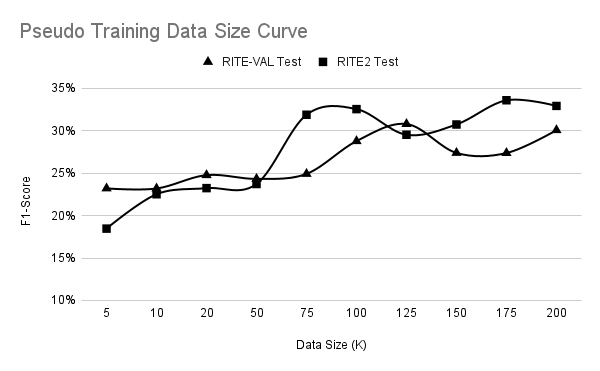
\includegraphics[width=15cm]{PseudoTrainingDataSizeCurve.png}
  \caption[Pseudo Training Data Size Curve]{The relationship between pseudo training data size and the performance of the recurrent neural network}
  \label{fig:pseudo_datasize}
\end{figure}

% 我們將虛擬訓練資料章節所產生的虛擬資料用來訓練 BERT,並且以 RITE 資料集做微調,也嘗試將虛擬資料與 CNLI 資料集混合在一起做為不同的訓練資料來測試其效能,其結果如表。在規則式虛擬資料與 CNLI 資料集混合的實驗中,其效能高於只用 CNLI 資料集做為訓練資料的實驗。
\paragraph{}
We use the pseudo training data as the pretraining dataset to train BERT and fine-tune it with the RITE dataset. We also try to mix the pseudo dataset with the CNLI dataset to see the performance. The results are shown in Table \ref{result:pseudo_nli_bert}. We can see the performance of the rule-based pseudo dataset is better than the GPT-2 pseudo dataset, and the performance of rule-based pseudo dataset mixed with the CNLI dataset is better than the performance of the CNLI dataset.

\begin{table}[H]
  \centering
  \setlength{\extrarowheight}{-3pt}
  \caption{Results of the BERT that train with Pseudo-NLI and fine-tune with RITE.}
  \label{result:pseudo_nli_bert}
  \begin{tabular}{|l|l|l|l|l|}
  \hline
  \multicolumn{1}{|c|}{\multirow{2}{*}{Dataset}} & \multicolumn{2}{c|}{RITE-VAL} & \multicolumn{2}{c|}{RITE2} \\ \cline{2-5}
  \multicolumn{1}{|c|}{} & \multicolumn{1}{c|}{Dev} & \multicolumn{1}{c|}{Test} & \multicolumn{1}{c|}{Dev} & \multicolumn{1}{c|}{Test} \\ \hline
  Rule-Based   Pseudo-NLI & \textbf{0.5524} & 0.4257 & 0.6541 & \textbf{0.5777} \\ \hline
  GPT-2   Pseudo-NLI & 0.5156 & 0.4210 & 0.6283 & 0.5378 \\ \hline
  Half   Pseudo-NLI & 0.5255 & 0.4276 & 0.6440 & 0.5462 \\ \hline
  All   Pseudo-NLI & 0.5258 & \textbf{0.4440} & \textbf{0.6695} & 0.5659 \\ \hline \hline
  CNLI-TW & 0.5915 & 0.5146 & 0.6848 & 0.6426 \\ \hline
  Rule-Based   Pseudo-NLI + CNLI-TW & 0.5992 & \textbf{0.5423} & 0.6908 & \textbf{0.6710} \\ \hline
  GPT-2   Pseudo-NLI + CNLI-TW & 0.5964 & 0.5364 & 0.6687 & 0.6409 \\ \hline
  Half   Pseudo-NLI + CNLI-TW & 0.5858 & 0.5317 & 0.6881 & 0.6572 \\ \hline
  All   Pseudo-NLI + CNLI-TW & \textbf{0.6114} & 0.5335 & \textbf{0.6940} & 0.6595 \\ \hline
  \end{tabular}
\end{table}

% 承諾會在口試後跑完的東西
\paragraph{(Upcoming Work)}
預計以\ MNLI 資料集為基底進行綜合型的實驗比較,將所有提到的實驗方法融合進去,並追加\ Pseudo-NLI 結合\ ML Features 與\ SWS 的實驗,期望能在論文定稿之前跑出實驗結果。

\subsection{Miscellaneous}
% 我們比較了在使用 CNLI 資料集作為訓練資料時,有沒有使用 WAG 與 MLFT 的效能。
\paragraph{}
We compare the performance of the recurrent neural network whether to use the similarity-based word sequence and the machine learning features. We use the CNLI dataset as the training data. The results are shown in Table \ref{result:rnn_cnli}. We can see that the similarity-based word sequence and the machine learning features have huge improvements when using a ten thousand level dataset.

\begin{table}[H]
  \centering
  \setlength{\extrarowheight}{-3pt}
  \caption{Using CNLI as training data in the recurrent neural network experiments.}
  \label{result:rnn_cnli}
  \begin{tabular}{|l|l|l|l|l|}
  \hline
  \multicolumn{1}{|c|}{\multirow{2}{*}{System}} & \multicolumn{2}{c|}{RITE-VAL} & \multicolumn{2}{c|}{RITE2} \\ \cline{2-5}
  \multicolumn{1}{|c|}{} & \multicolumn{1}{c|}{Dev} & \multicolumn{1}{c|}{Test} & \multicolumn{1}{c|}{Dev} & \multicolumn{1}{c|}{Test} \\ \hline
  RAD & 0.3314 & 0.2710 & 0.2849 & 0.2926 \\ \hline
  RAD + SWS + MLFT & \textbf{0.4601} & \textbf{0.3762} & \textbf{0.4847} & \textbf{0.4643} \\ \hline
  \end{tabular}
\end{table}

\section{Conclusion} \label{section:conclusion}
\paragraph{}
% 文意蘊含系統在自然語言領域裡是相當核心的技術,藉由深度學習的方法,大幅降低了過去特徵工程的複雜性,而讓研究者可以更專注於在適當領域的文本探勘,並借助遷移式學習的力量,將資源與成果較為豐富的語言轉移到相對弱勢的繁體中文上。
Textual entailment recognizing system is a quite core technology in natural language processing. The complexity of feature engineering is significantly reduced by deep learning and the researchers can focus more on the data mining of the proper domain. And with the help of transfer learning, the language with rich resources can apply the result on the Traditional Chinese which is relatively weak in resources.

\paragraph{}
% 本論文主要提出三種系統,第一種是使用 Sentence-based features 的機器學習,第二種是綜合了 Sentence-based features, Word-based sequence features 與 WGA 三種特徵的 Neural Network,第三種是使用了 Cross-lingual Transfer Learning 的 Transformers BERT。其中使用了 Cross-lingual Transfer Learning 的 Transformers BERT 讓我們將 RITE 資料集的實驗推向深度學習的領域且實現了相當卓越的效能。
In this thesis, the best of our systems is the transformers BERT using cross-lingual transfer learning. This system lets us push the experiments of RITE datasets to the field of deep learning and achieved quite excellent performance.

\paragraph{}
% 在資料集改善的方面,除了 Reversed Labels 與資料集混合以外,我們也提出了使用 GPT-2 產生虛擬訓練資料的方法,透過實驗證實了這個方法有一定程度的效果,我們認為這個方法也相當具有潛力。未來若是有更強大的運算效能可以將這個實驗套用到 GPT-2-LARGE 或 GPT3 上可能會有更好的結果。
In the experiments of training data expansion, in addition to reversed labeling and mixing datasets, the pseudo training data generated by rule-based and GPT-2 is proposed. We proved this method is effective. We think this method is quite potential. In the future, with more powerful computing performance, the GPT-2-LARGE or GPT3 may be applied to the experiments and may get better performance.

\paragraph{}
% 核心模組皆為開源系統,本論文的實驗都具有高度的可重製性。我們希望這樣的研究方向與經歷可以提供給其他資源也同樣相對匱乏的語言的研究者一個參考。
Our core modules are open-source systems and our experiments are highly reproducible. We hope this research direction and experience may provide a reference for other research in the language which is also relatively low resources.

\end{spacing}

\addcontentsline{toc}{section}{References}
\bibliography{main}
\bibliographystyle{unsrtnat}
% \printbibliography
\end{CJK*}
\end{document}
